


\chapter{Variáveis aleatórias regionalizadas} \label{cap_var_reg}

\begin{myquoting}{Kato Lomb}
	
	Todas as vezes que eu leio relatórios estatísticos, eu tento imaginar meu contemporâneo infortunado, a Pessoa Média, a quem, de acordo com estes relatórios, possui 0.66 filhos, 0.032 carros e 0.046 TVs. 
	
\end{myquoting}

\section{Introdução ao capítulo}

A geoestatística é uma ciência que se inicou nos anos de 1950, com estudos de \citet{krige1960departure}  na África do Sul a respeito de valores estimados em distribuições lognormais de ouro. Em 2012 o professor Daniel Krige recebeu a Ordem de Baobab, uma condecoração do presidente da África do Sul, pelas suas excepcionais contribuições para a economia, ciência, medicina, inovações tecnológicas e serviços comunitários. Durante seus 30 anos de idade,  se tornou pioneiro no uso da estatística para avaliação de depósitos de ouro para um número limitado de furos de sondagem. As ideias do pesquisador foram fortemente abraçadas pela França após a tradução de seus artigos em língua nativa em 1995, o que gerou a fundação do centro de Geoestatística em Fontainebleau, corroborando para os estudos do professor George Matheron, e a criação da \textbf{teoria das variáveis regionalizadas}.


 Este primeiro capítulo introduz a geoestatística a partir do seu objeto de estudo, as variáveis regionalizadas. Explicamos os principais conceitos abordados pela teoria clássica, e como eles se relacionam no entendimento dos fenômenos espacializados. Maiores informações podem ser encontradas nas obras de Matheron \cite{matheron1963principles} ou nos livros base de \cite{isaaks1989applied} e \cite{goovaerts1997geostatistics}


\section{Variáveis aleatórias} 

Alguns conceitos iniciais sobre estatística são necessários antes que possamos aprofundar os conceitos de geoestatística. Um dos principais conceitos utilizados para o entendimento de fenômenos aleatórios é o de \textbf{variável aleatória}. 

\begin{definition}[Variável aleatória] 
	\textit{Uma variável aleatória é uma função de um espaço amostral S nos números reais.} \citet{casella2010inferencia}
\end{definition} 

Imagine que tenhamos um saco com grandes quantidades de pedras coloridas vermelhas e azuis. Nosso espaço amostral seria portanto \textbf{S=\{pedras vermelhas, pedras azuis\}}. Se quisermos determinar uma variável aleatória que seja definida pela amostragem de duas pedras poderíamos ter o seguinte resultado \textbf{Z =\{(pedra vermelha, pedra azul) , (pedra vermelha, pedra vermelha), (pedra azul, pedra azul)\}}. Uma variável aleatória geralmente é definida a partir de uma letra maiúscula, enquanto uma realização, ou seja, um resultado desta variável aleatória é definido por uma letra minúscula. A figura \ref{Indicadora} é um exemplo de uma variável aleatória, pois para cada valor possível dentro do espaço amostral de diferentes litologias é associado um valor inteiro. 

\FloatBarrier
\begin{figure}[!htb]
	\centering
	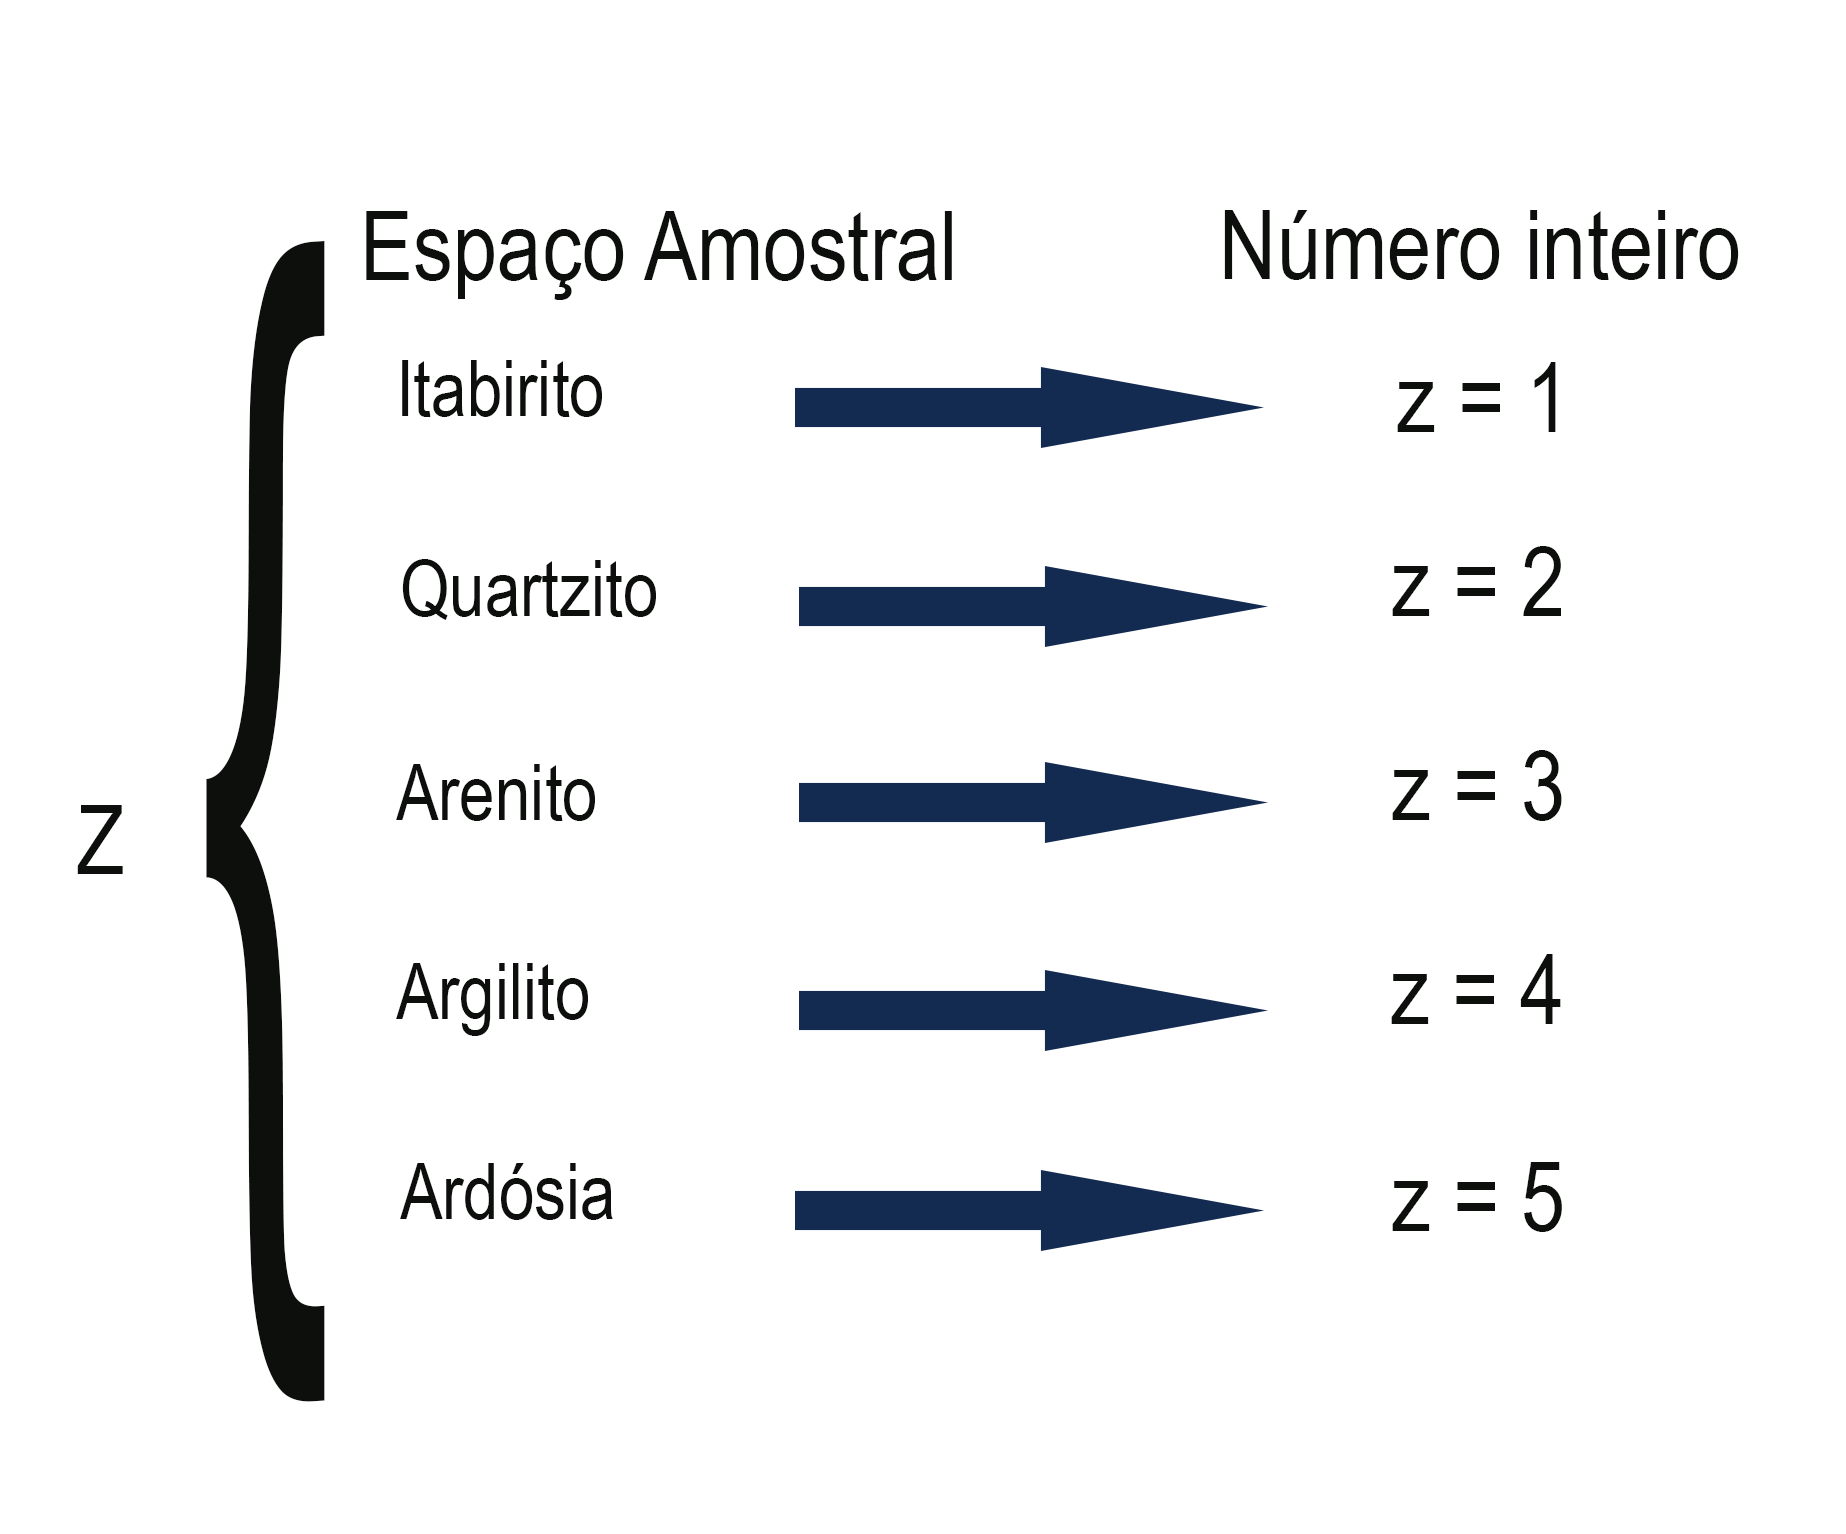
\includegraphics[scale=0.7]{./Capitulo_1/Indicadora.png}	
	\caption{Exemplo de variável aleatória indicadora. Para cada possível valor de litologia do depósito é associado um valor inteiro. }
	\label{Indicadora}
\end{figure}
\FloatBarrier

Note, no entanto, que atribuir um valor para esta variável não significa dar uma maior importância ou uma menor importância para cada litotipo. Colocar um valor inteiro igual a 1 para o Itabirito não significa considerá-lo mais importante que as demais litologias. Neste caso dizemos que esta variável é \textbf{cardinal}, pois o valor associado de cada componente do espaço amostral a um valor inteiro não está diretamente ligado com sua importância, ao contrário de variáveis \textbf{ordinais} ao qual seu número associado é diretamente expresso pela sua importância.

 As variáveis aleatórias são divididas geralmente em duas classes na geoestatística, considerando \textbf{variáveis aleatórias reais}, que podem apresentar valores dentro do conjunto de dados reais, ou \textbf{variáveis indicadoras}, quando consideramos que podem assumir valores inteiros. Exemplos de variáveis reais, por exemplo, são as de teores dos elementos metálicos, enquanto variáveis indicadoras são representadas pelas litologias presentes no depósito mineral. 
 
 Variáveis ditas \textbf{contínuas} são aquelas que possuem um espaço amostral infinito e  \textbf{não contável},  geralmente representada por um conjunto de valores reais. Quando medimos teores, por exemplo, o resultado de uma amostra pode variar infinitamente dentro de um intervalo de 0\% a 100\%. Apesar desta limitação, o número de realizações que podem advir desta variação são infintas, pois naturalmente o valor 5,6740 \% é diferente do valor 5,6741 \%, mesmo que muito próximos.
 
 Em contrapartida, variáveis discretas são \textbf{contáveis}, mesmo que seu espaço amostral seja infinito. Se um subconjunto deste espaço amostral for considerado é possível conseguir definir para ele uma probabilidade. Variáveis discretas estão geralmente ligadas ao conjunto de números inteiros.
 
  Para uma variável aleatória pode ser atribuído uma probabilidade $(Pr)$ de ocorrência para cada uma de suas realizações. A ideia de probabilidade mais básica está relacionada com a \textbf{frequência de ocorrência relativa de um evento}, ou também chamada de abordagem frequentista. Nossa variável aleatória demonstrada pela figura \ref{Indicadora} pode ser associada a uma probabilidade de acordo com a figura \ref{Prob}, considerando a proporção de rochas de cada tipo dentro do domínio geológico estimado. 
  
  \FloatBarrier
  \begin{figure}[!htb]
  	\centering
  	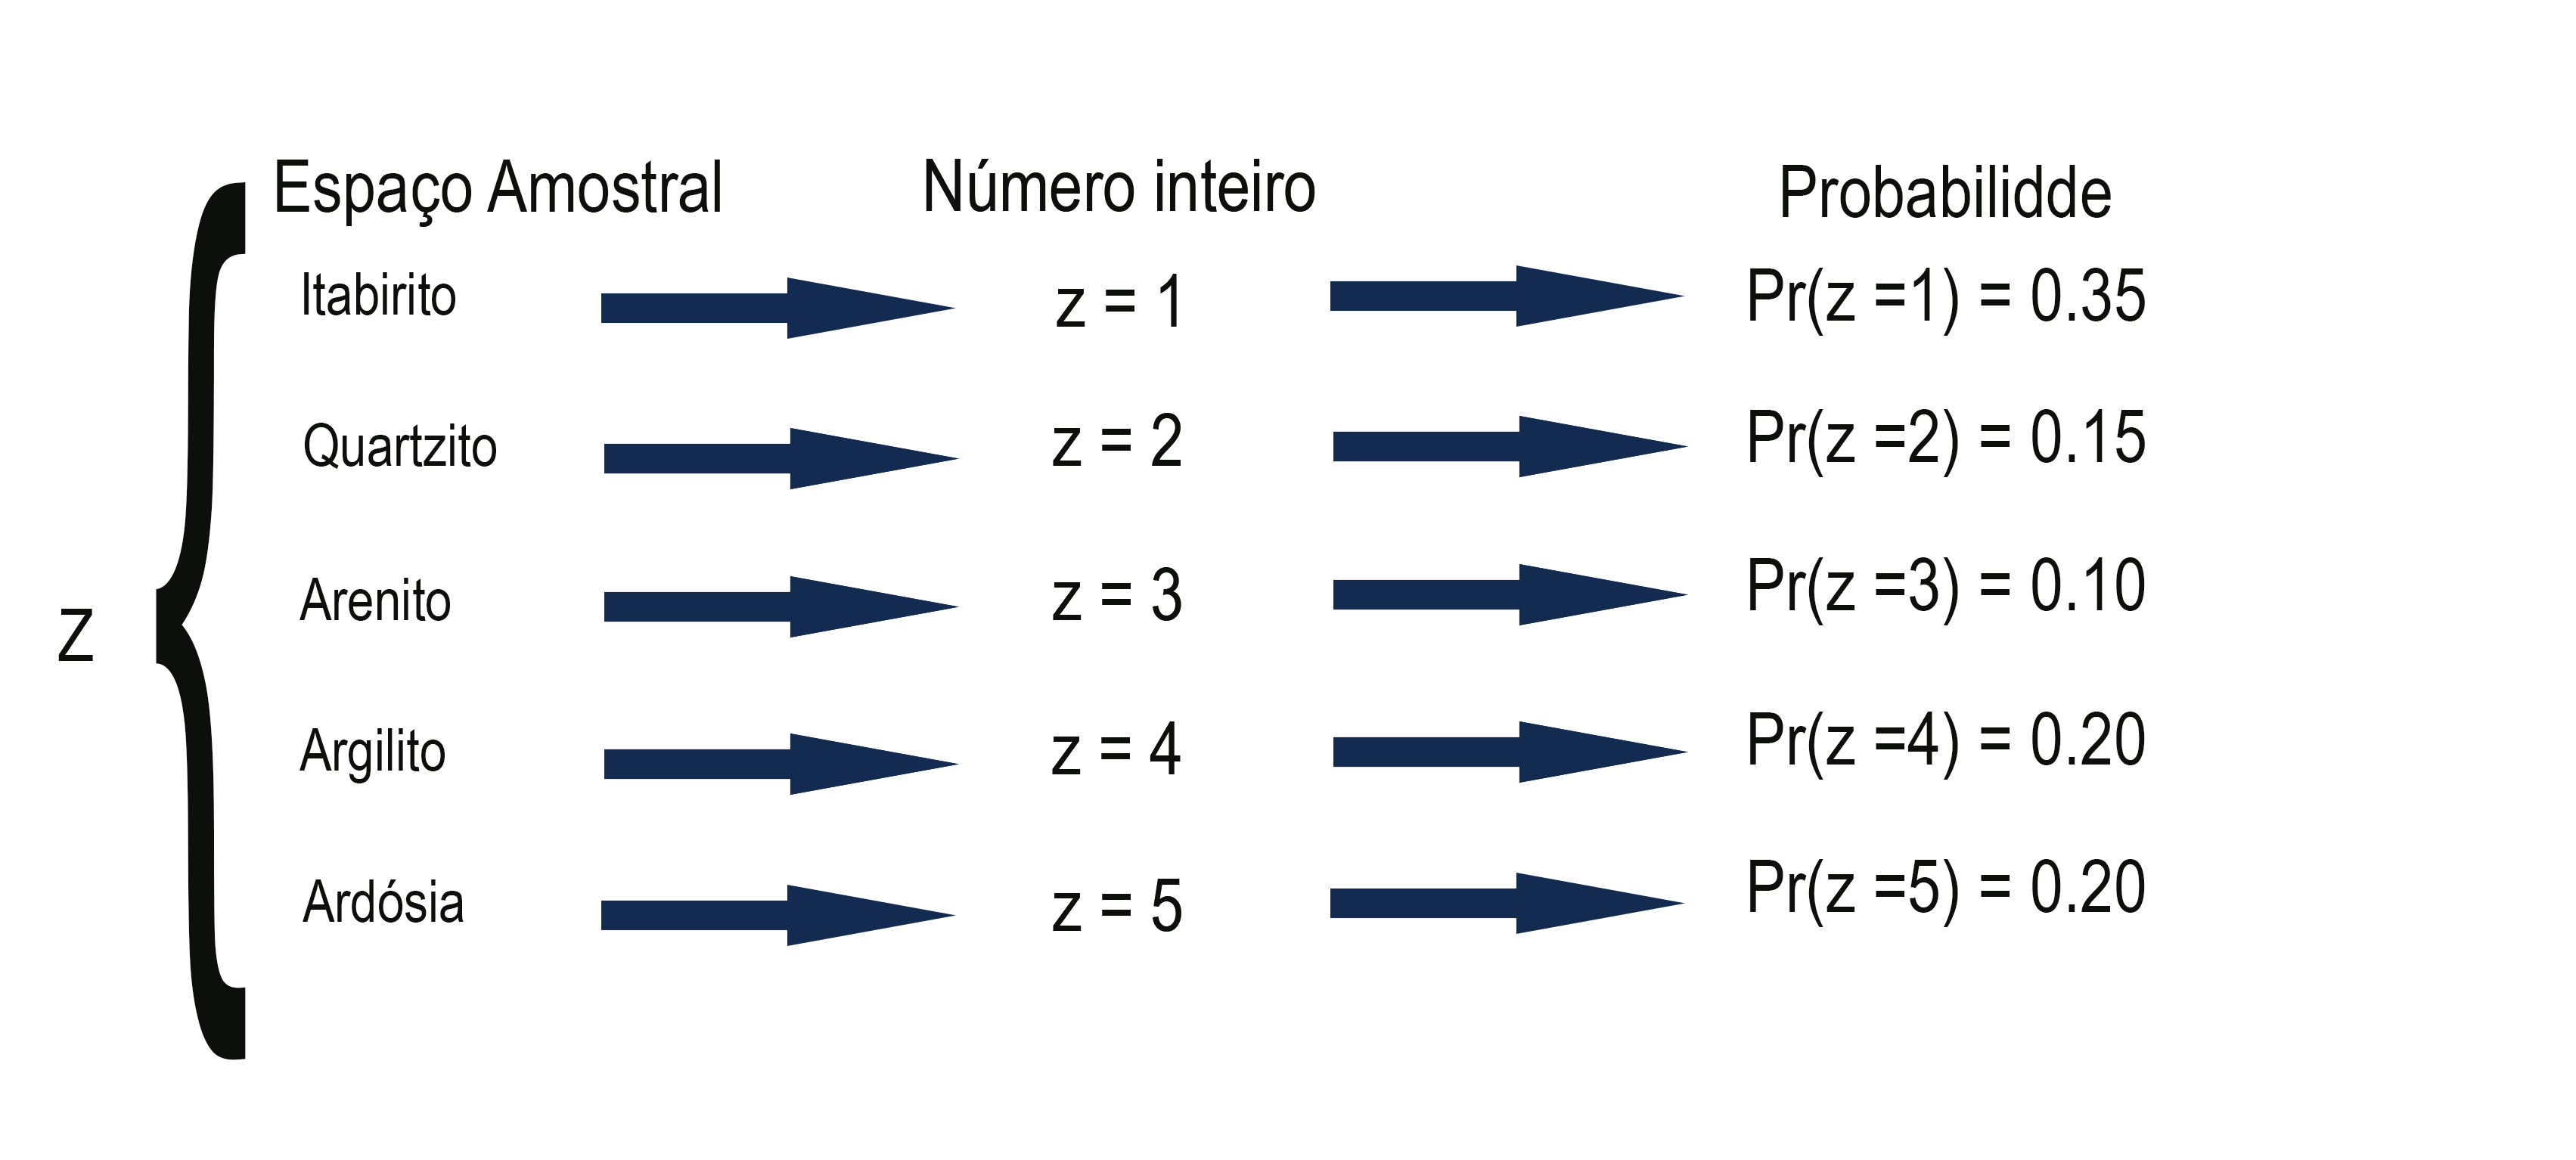
\includegraphics[scale=0.7]{./Capitulo_1/Prob.png}	
  	\caption{Exemplo de variável aleatória indicadora. Para cada possível valor de litologia do depósito é associado um valor inteiro. Uma probabilidade é atribuída para a frequência relativa de cada litologia. }
  	\label{Prob}
  \end{figure}
  \FloatBarrier
  
  Em outras palavras a probabilidade é semelhante a uma métrica de proporção das realizações de uma variável aleatória. Na verdade a probabilidade pode ser qualquer medida, desde que satisfaça os \textbf{Axiomas de Kolmogorov}. 
  
  \begin{enumerate}
  	\item A probabilidade de um evento é um número não negativo, dentro do intervalo [0,1].
  	\item A probabilidade do espaço amostral é 1.
  	\item Se n eventos são mutuamente exclusivos, a probabilidade da união destes eventos é igual a soma das probabilidades individuais.
  \end{enumerate}
  
    Os conceitos de probabilidade são estudados na matemática dentro da \textbf{teoria dos conjuntos}  que é a base para a fundamentação da estatística. Para maiores informações da teoria base em probabilidade, axiomas de Kolmogorov e teoria dos conjuntos, aconselhamos ler as referências de \citet{alencar2014teoria} e \citet{feitosa2011teoria}.
 
 \section{Função de distribuição acumulada - fda}  
 
Para cada elemento de uma variável indicadora podemos associar um valor de probabilidade, ou de frequência da apresentação deste elemento. Por exemplo se consideramos que um depósito mineral possui apenas dois tipos de rocha, podemos dizer que o tipo 1 representa 30\% de frequência no depósito mineral, enquanto o tipo 2 apresenta 70\% de frequência. Associar uma probabilidade para variáveis aleatórias indicadoras é intuitivo. No entanto, não conseguimos definir a probabilidade de um elemento para variáveis aleatórias reais contínuas, pois o espaço amostral é infinito. Não conseguimos associar, por exemplo, a probabilidade de um teor ser 5,67\%. Neste caso utilizamos uma abordagem intervalar, associando a probabilidade a um intervalo de valores reais, logo é possível dizer que o depósito mineral possui probabilidade de 40\% dos teores variarem de 5,67\% a 9,32\%. Uma função de distribuição acumulada é representada pela probabilidade de uma variável aleatória assumir um valor igual ou menor a um determinado limite. Definimos então a \textbf{Função de distribuição acumulada $F(z)$} tal como  

\begin{equation}
F(z) = \Pr(Z \leqslant z)
\end{equation}

A figura \ref{distribuicoes} indica a função de distribuição para variáveis contínuas e discretas. Em A) possuímos uma função discreta que pode assumir apenas valores inteiros de 1 a 8. Em B) possuímos uma função contínua de valores que se alteram no intervalo [1,8]
	
	
\FloatBarrier
\begin{figure}[!htb]
	\centering
	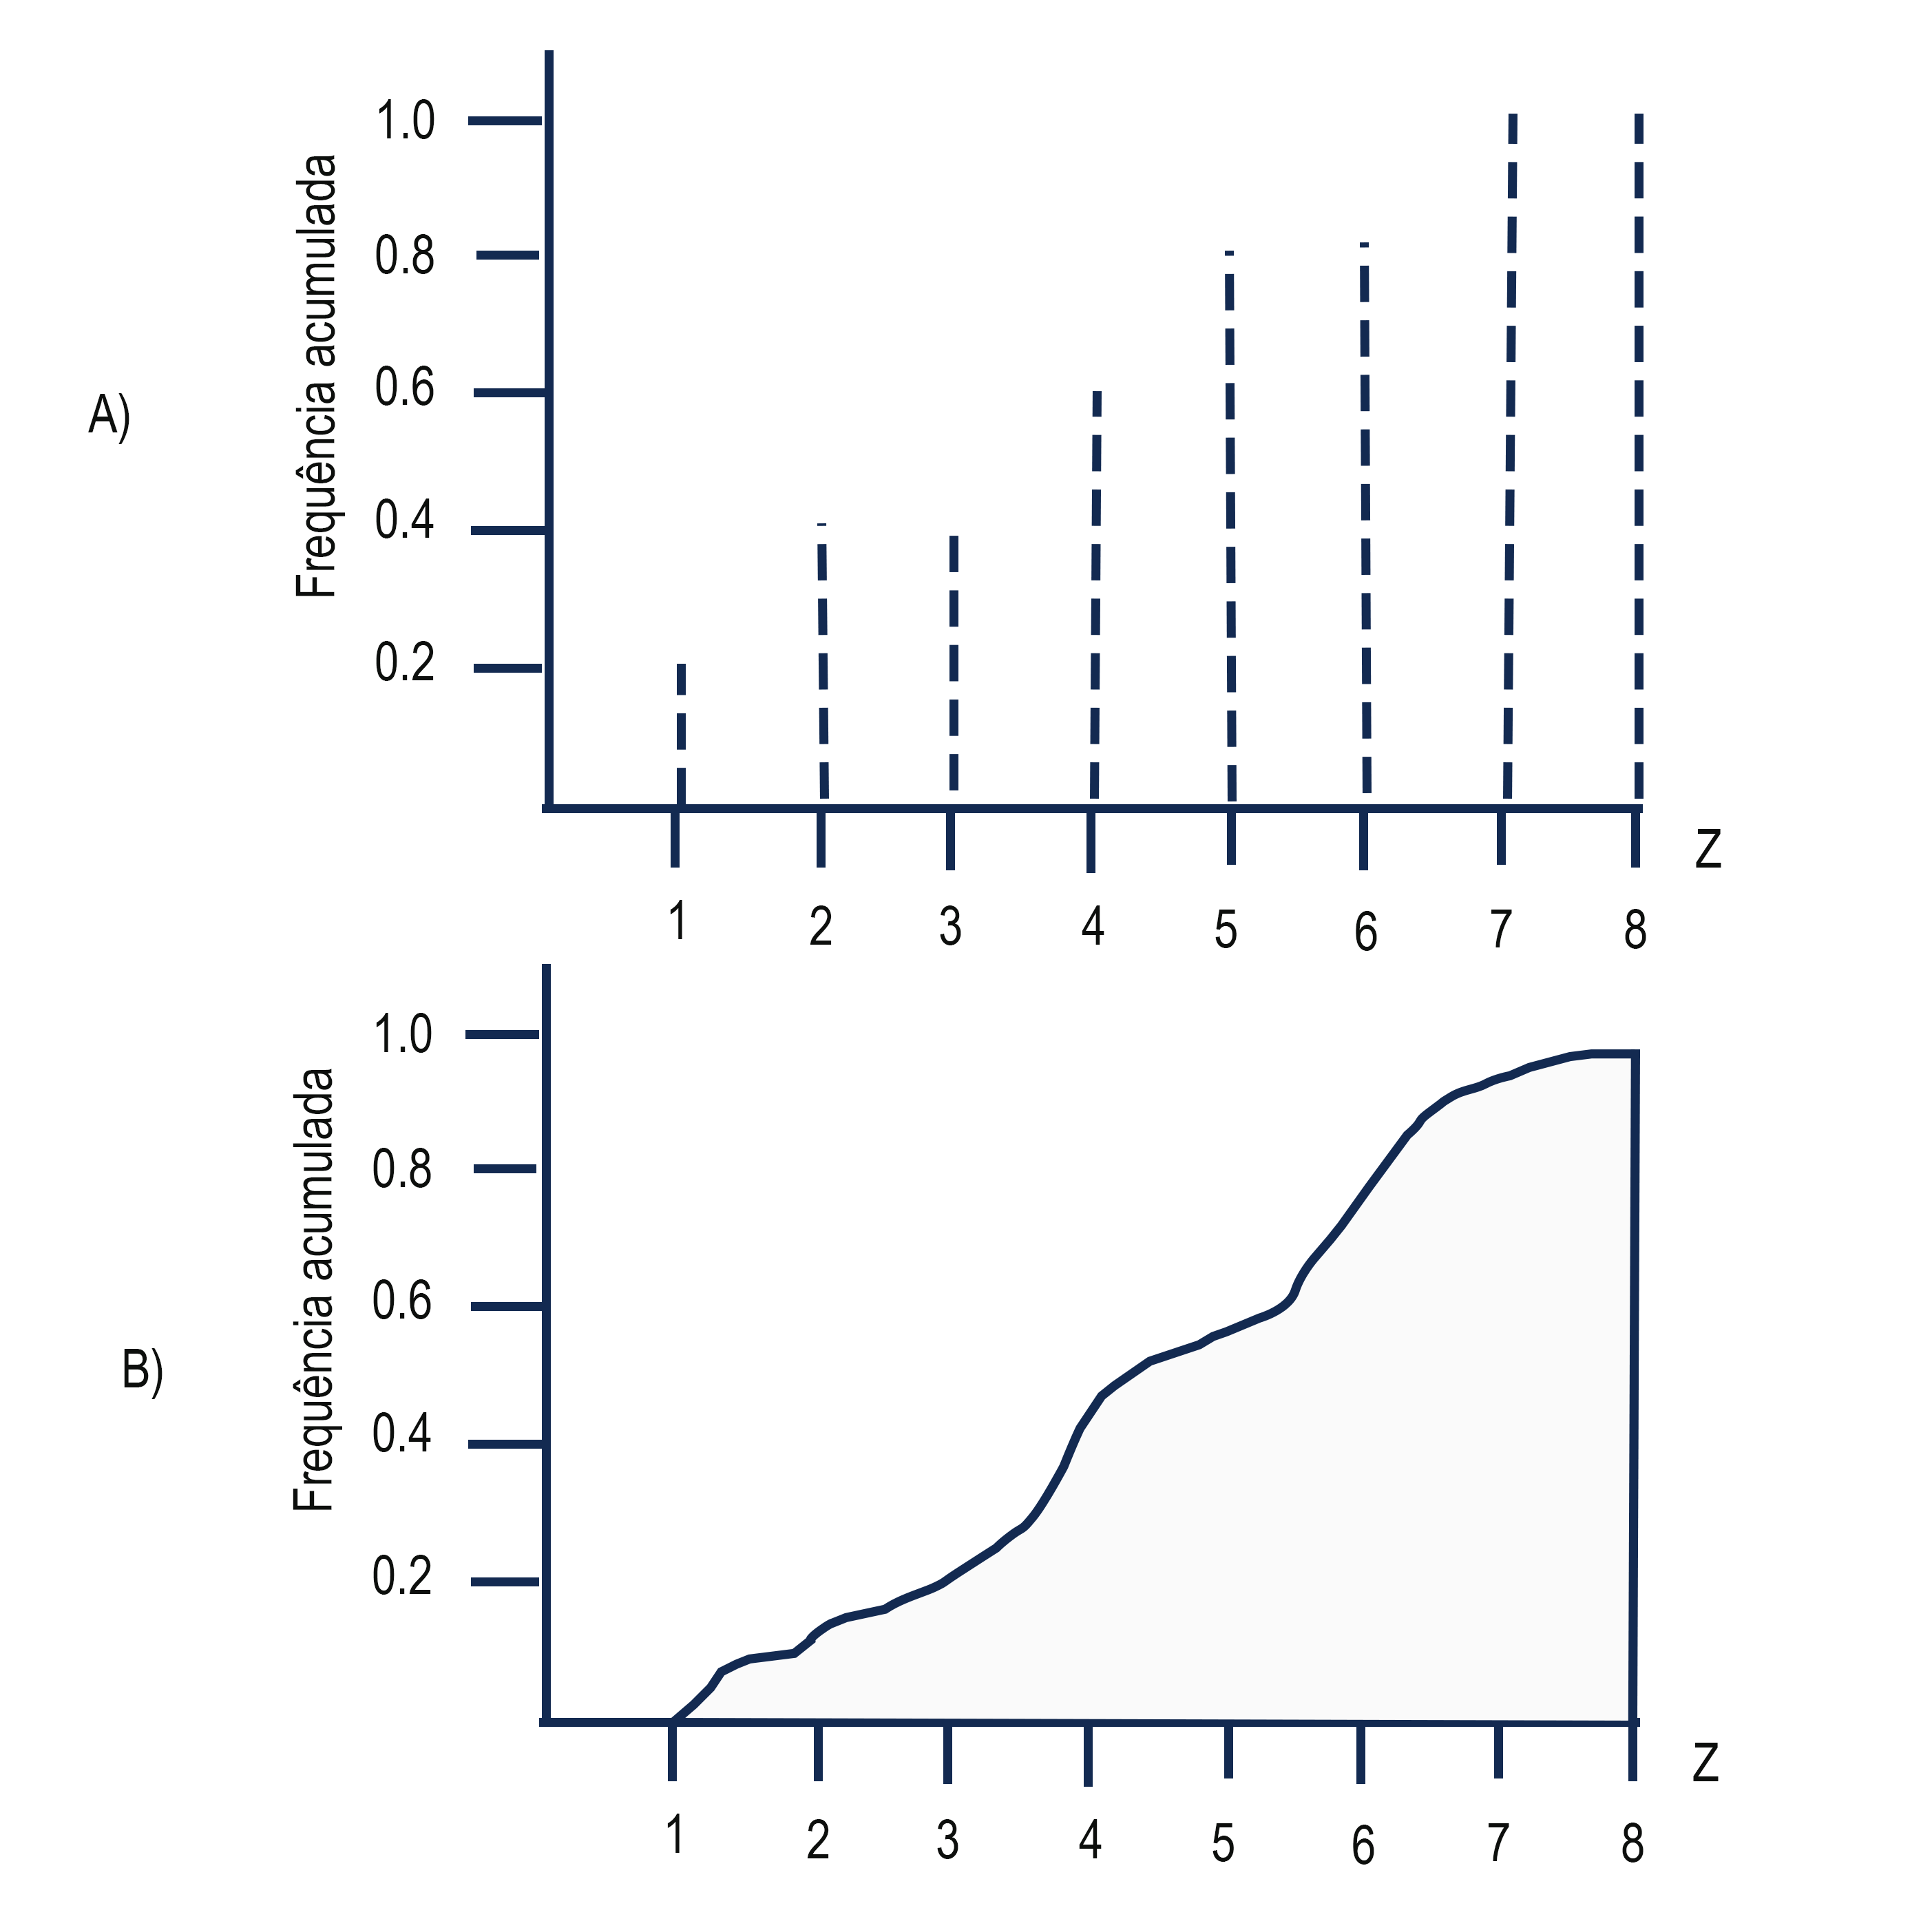
\includegraphics[scale=0.5]{./Capitulo_1/Distribuicoes.png}	
	\caption{Função de distribuição acumulada - fda para variáveis discretas A) e contínuas B) }
	\label{distribuicoes}
\end{figure}
\FloatBarrier

\section{Função de densidade de probabilidade - fdp}  

No caso de distribuições contínuas, em que os valores podem ser determinados para qualquer valor dentro de um domínio real, é permitido utilizar princípios de cálculo para medir informações dessas distribuições. Como não podemos definir o valor da probabilidade em um ponto específico precisamos utilizar o conceito de probabilidade intervalar. A \textbf{Função de densidade de probabilidade-fdp} pode ser determinada como a probabilidade um valor assumir este valor dada uma variação infinitesimal.

\begin{equation}
f(z) = lim_{\delta \rightarrow 0}\left [ Pr(Z > z, Z < z + \delta ) \right ]
\end{equation}

Logo a relação entre a função de distribuição acumulada e a função de densidade de probabilidades pode ser expressa por 

\begin{equation}
F(z) = \int_{-\infty }^{z} f(z) dz
\end{equation}

\begin{proposition}
	\textit{Pode parecer que o valor da densidade de probabilidade seja equivalente ao valor da probabilidade assumindo uma realização $z$ de variável aleatória $Z$, no entanto esta visão está errada! A ideia de probabilidade está diretamente ligada na ideia de frequência relativa de um evento. Valores de variáveis contínuas possuem espaço amostral incontável, o que significa que não conseguimos medir o seu tamanho, sendo ele infinito. Quantos seriam os possíveis resultados, por exemplo, de um teor de uma amostra apresentar? Se fosse possível associar uma probabilidade a um valor de uma variável aleatória real, todos estes valores seriam iguais a zero, pois sua frequência em nada representa na imensidão de valores possíveis. A função de densidade de probabilidade é na verdade uma medida de taxas de variação da probabilidade.}
\end{proposition}

\section{Variáveis regionalizadas} 

\citet{matheron1963principles} , pai fundador da geoestatística, iniciou o conceito de \textbf{variável regionalizada}, para exemplificar os fenômenos espaciais. Quando um fenônmeno exibe uma certa \textbf{estruturação espacial}, dizemos ele ser regionalizado. Os fenômenos geológicos, por exemplo, exibem estruturação característica na sua formação, o que significa que os corpos geológicos apresentam geometrias características de suas gêneses. A variável regionalizada $z(x)$ denota um valor conhecido em um determinado ponto $x$, sendo apenas um resultado neutro puramente descritivo, sem interpretação probabilística. Em outras palavras, a variável regionalizada é o valor real encontrado no depósito mineral para cada ponto $x$ no espaço. 

\begin{definition}[Variável Regionalizada]
	\textit{Uma variável regionalizada $z(x)$ representa a medida de uma propriedade qualquer, seja ela o teor do elemento metálico, quantidade de metal ou acumulação, definida em um ponto $x$ no espaço de coordenadas definidas}
\end{definition}

É impossível para nós conhecer o valor real de $z(x)$ para cada ponto no espaço, pois implicaria em muito mais que uma amostragem sistemática por todo o domínio do depósito mineral. Desta forma a variável regionalizada apresenta aspectos contraditórios, porém complementares para a definição do modelo geoestatístico:

\begin{itemize}
	\item \textbf{Apresenta uma componente aleatória} onde não conseguimos amostrar ou definir a variável. Isto marca o aspecto irregular da variável. Seguindo a notação estatística, nos locais onde a variável regionalizada não é definida, denotamos $Z(x)$ para informar que nestes locais ela assume aspecto de uma variável aleatória. Sendo $\Omega$ o universo que pode ser composto a variável, definimos a variável aleatória em local desconhecido da variável regionalizada como $Z(x):\Omega \rightarrow \Re $.
	\item \textbf{Apresenta uma componente estruturada} nos locais onde é determinada, como por exemplo, pelos métodos de amostragem, representada pela própria forma $z(x)$, convencionalmente pela notação estatística como a realização da variável aleatória $Z(x)$ no suporte $x$. 
\end{itemize}

\begin{proposition}
	\textit{Pode parecer um tanto estranho que algo possa assumir condições dicotômicas desta forma. Ao mesmo tempo que consideramos que algo existe e é determinístico, também consideramos que algo é aleatório e transitório. Na verdade as coisas são como sempre são, o que fazemos é assumir que em certos casos, não conseguimos definir algo, e em outro sabemos muito bem o que é. A aleatoriedade, na verdade, nunca existiu. Aleatoriedade é nosso princípio de humildade em não entendermos como os fenômenos ocorrem.}
\end{proposition}

A observação da variável regionalizada, não ocorre, no entanto em um ponto do espaço. Pontos são abstrações matemáticas de dimensão infinitesimal, uma condição geralmente para que possamos aplicar o princípio de continuidade dos modelos. As nossas observações são realizadas em amostras com volumes específicos e em grandes regiões que queremos estimar. \citet{matheron1963principles} apresenta os principais conceitos de domínio e suporte. Um domínio é uma região onde a variável regionalizada é diferente de zero. No nosso livro apresentamos o domínio das estimativas pela notação $D$, enquanto os domínios de um bloco ou painel de lavra são apresentados por $V$.


\begin{definition}[Domínio]
	\textit{Domínio de uma variável regionalizada pode ser considerada qualquer região onde a variável apresenta valor diferente de zero. Por exemplo, a região da mina onde pretendemos estimar valores desconhecidos pode ser considerada como um domínio de estimativa D.}
\end{definition}

\citet{matheron1963principles} apresenta também o conceito de suporte,  sendo este relacionado com a capacidade de entendimento da variável regionalizada $z(x)$. De certa forma, é impossível conhecer o valor da variável regionalizada em um ponto $x$, pois o que detemos é o conhecimento da variável em um volume $v$, representando um testemunho de rocha, ou um fragmento de rocha. 

\begin{definition}[Suporte]
	\textit{Suporte é o volume e forma $v$ ao qual se detém o conhecimento da variável regionalizada $z_{v}(X)$}
\end{definition}

Em alguns casos, pela dimensão do domínio estimado em relação ao suporte, este é quase observado como um ponto. Imagine um framento de rocha de $10cm^{3}$ e um painel a ser estimado de $200m^{3}$. A diferença de ordem de grandeza entre a amostra e o painel é gigantesca.

\begin{proposition}
	\textit{Dizemos que do ponto de vista matemático é quase impossível definir a variável regionalizada $z(x)$, pois é quase impossível amostrar em um ponto. No entanto, esta é uma observação muito purista, que desconsidera os aspectos de engenharia. Em alguns casos uma amostra pode ser visualizada como uma realização da variável regionalizada $z(x)$, pois o volume da amostra é tão inferior ao domínio, que se torna praticamente uma dimensão pontual}
\end{proposition}

Uma das condições de aplicação da geoestatística clássica, que considera o uso de variáveis aditivas, é que o suporte das amostras utilizado nas estimativas deve ser o mesmo. Isto significa que o volume dos testemunhos utilizados para estimativa, amostras de canais, ou outros tipos de amostragens devem ter todos mesma forma, tamanho e volume. Esta é também outra questão impraticável, pois é impossível principalmente em rochas, obter regularidade nas amostras desta forma. Para contornar esta situação nos utilizamos os métodos chamados de \textbf{regularização}, que permitem criar amostras de mesmo tamanho. 



Estas definições são as clássicas paresentadas pelo professor George Matheron em seus primeiros trabalhos sobre a teoria das variáveis aleatórias regionalizadas. Existe muita confusão entre diferentes autores para a representação destes conceitos de \textbf{suporte} e \textbf{domínio}, sendo muitas vezes o domínio do painel chamado de suporte do painel. De acordo com a definição de suporte, seria necessário conhecer o valor real do painel, o que é impossível, sendo mais adequada a nomeclatura de domínio do painel. Estas divergências de conceituação não prejudicam o estudo da geoestatística como um todo, mas acabam por criar diferentes formas de notação e algumas vezes dificultam a leitura dos textos. O mais importante em se ter em mente é que este volume, seja do domínio ou do suporte, pode alterar os resultados das suas estimativas, na chamada \textbf{relação volume e variância}.



Esta ambiguidade da variável regionalizada permite tratamento de forma diferenciada segundo os objetivos de cada estudo. Podemos, ora tratar a variável regionalizada apenas como valores dispostos no espaço, ora dar um tratamento probabilístico para estes valores. \citet{matheron1963principles} aborda estes dois princípios como 

\begin{itemize}
	\item \textbf{Métodos transitivos} Considera a hipótese de estacionaridade, mas não implica em qualquer hipótese probabilística, sendo métodos apenas descritivos da variável regionalizada $z(x)$. Esta abordagem é utilizada principalmente na geoestatística clássica abordada neste livro. Faremos os cálculos geoestatísticos considerando apenas a descrição dos valores amostrados em uma determinada região, sem premissas sobre uma possível distribuição de probabilidades local. 
	\item \textbf{Teoria intrínseca} Utiliza a intrepretação probabilística da variável regionalizada $Z(x)$, também considerando hipóteses de estacionaridade. Esta metodologia é amplamente utilizada nos métodos considerados não-lineares e nas simulações geoestatísticas, em que se pretende determinar não apenas um valor esperado determinístico para um volume estimado, mas também uma distribuição de probabilidades.  
\end{itemize}

\section{Funções aleatórias} 

Como dissemos anteriormente a variável regionalizada possui uma componente tanto determinística, onde conhecemos os valores da variável, como uma componente aleatória, em locais onde se desconhece a propriedade de interesse. Este aspecto dicotômico é trocado por alguns autores ao usarem da \textbf{teoria intrínseca} e estabelecerem a variável aleatória sobre termos exclusivos de uma interpretação probabilística.  Uma visão um pouco mais abstrata da variável aleatória é entender que sua componente determinística é apenas um resultado ou uma realização da variável aleatória naquele local, e que  $Z(x)$, chamada em alguns casos de \textbf{função aleatória} é uma função que associa a qualquer ponto do espaço uma variável aleatória.  A figura \ref{func_aleatoridade} demonstra o resultado de uma amostragem $z(x= x_{1})$ no ponto $x_{1}$.  


\FloatBarrier
\begin{figure}[!htb]
	\centering
	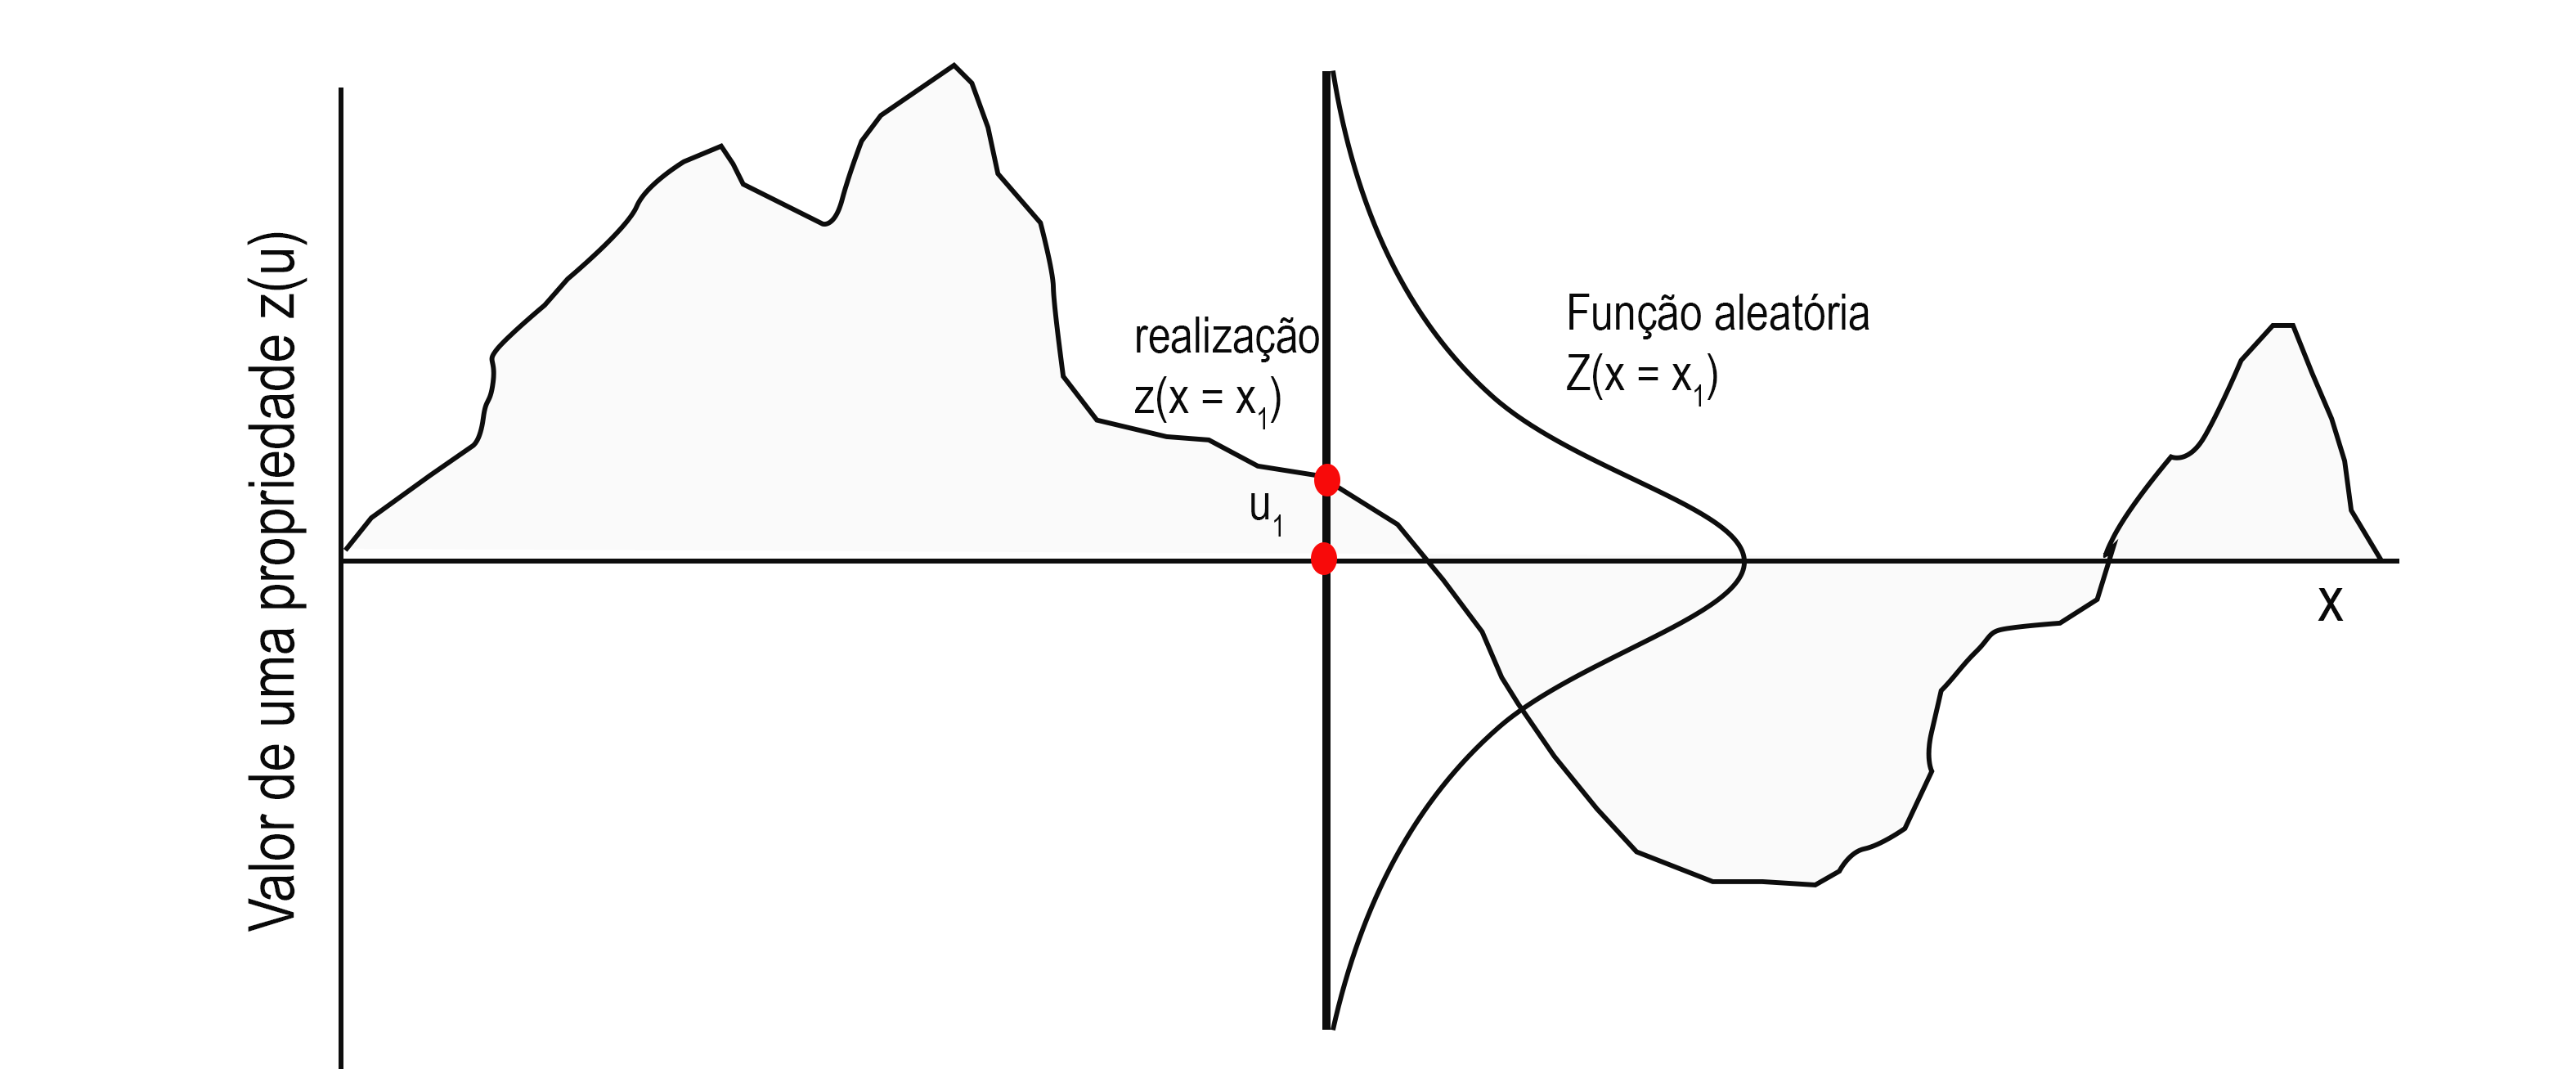
\includegraphics[scale=0.8]{./Capitulo_1/Variavel_aleator.png}	
	\caption{Demonstração do resultado amostrado $z(x = x_{1})$ como uma realização da função aleatória $Z(x = x_{1})$. No ponto $x_{1}$ o valor amostrado é apenas um resultado de uma função que desconhecemos, que associa uma distribuição de probabilidades naquele local. }
	\label{func_aleatoridade}
\end{figure}
\FloatBarrier

Em muitos os casos não é possível conhecer esta função geradora do depósito mineral, apenas tomamos como hipótese que ela existe e é uma combinação de variáveis aleatórias em todo o espaço. Na geoestatística muitas vezes consideramos que esta função pode ser representada como uma combinação linear destas variáveis, chamada de \textbf{geoestatística linear}, ou \textbf{geoestatística clássica}. Ao tomarmos esta simplificação proposta pela teoria intrínseca, a demonstração das técnicas geoestatísticas se tornam bem mais fáceis, por isso, durante este texto, pretendemos utilizar o conceito da função aleatória em vez da forma tradicional da variável regionalizada proposta por Matheron. 

\begin{definition}[Função aleatória]
	\textit{Uma função aleatória pode ser descrita como uma função que associa a cada ponto no espaço $x$ uma variável aleatória $Z(x =x_{1}))$, sendo $x_{1}$  o ponto de coordenas especificado. }
\end{definition}

Esta função aleatória é composta de uma amalgama de diversas variáveis aleatórias, cada uma em um ponto do espaço. A análise geoestatística destes valores permite decompormos esta função em duas componentes principais de acordo com os valores esperados de cada uma destas variáveis. O valor esperado tende a ser o de maior probabilidade de ocorrência em um determinado local. Desta forma podemos decompor a função aleatória em duas componentes principais, o \textbf{resíduo} e o valor de \textbf{tendência}. Por definição, a função aleatória pode ser expressa por $Z(x) = R(x) + m(x)$, sendo que os resíduos possuem média igual a zero.

\FloatBarrier
\begin{figure}[!htb]
	\centering
	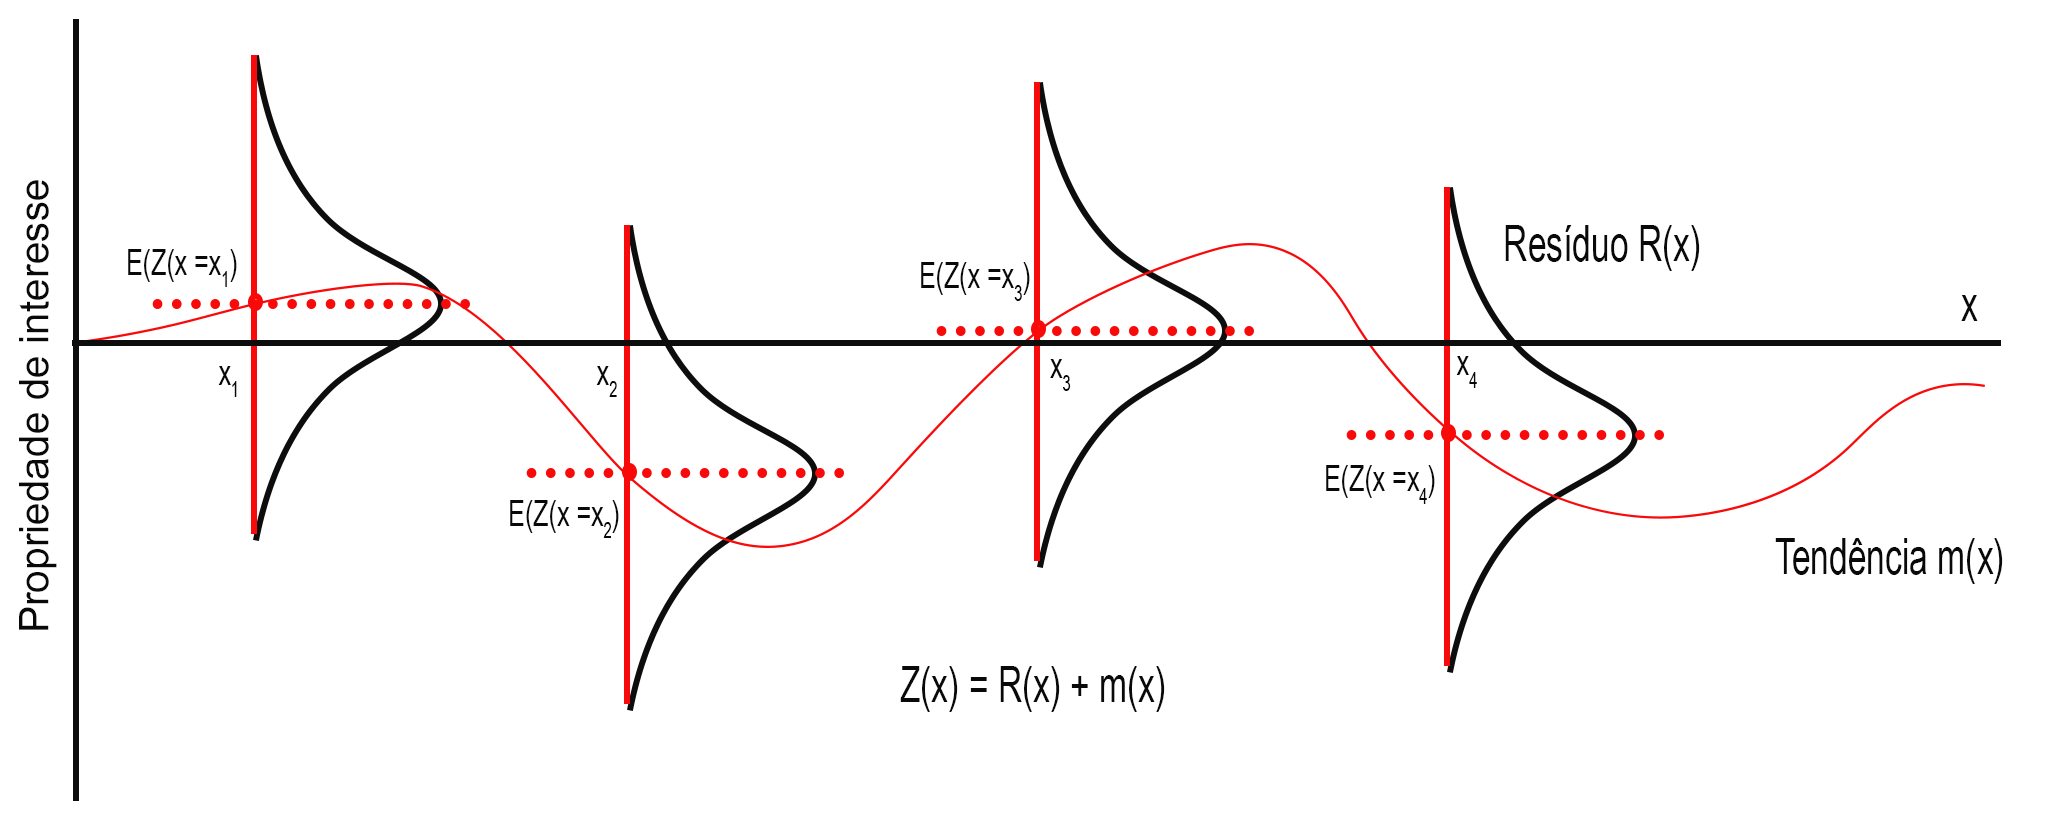
\includegraphics[scale=1]{./Capitulo_1/Decomp.png}	
	\caption{Decomposição da função aleatória a partir da determinação de sua tendência, indicada por $m(x)$, e o seu resíduo $R(x)$. }
	\label{decompos}
\end{figure}
\FloatBarrier


É comum na geoestatística assumirmos algumas hipóteses quanto a função aleatória. A \textbf{hipótese de estacionaridade de segunda ordem} afirma que o valor da tendência deve ser constante em todo o domínio considerado e o resíduo deve possuir variância constante para todo o domínio. Como desconhecemos a função aleatória, e nunca conseguimos determinar as variáveis aleatórias em cada ponto considerado, a hipótese de estacionaridade é sempre assumida, e nunca conseguimos comprová-la. Observe a série de números gerados na figura \ref{SerieA}. 

\FloatBarrier
\begin{figure}[!htb]
	\centering
	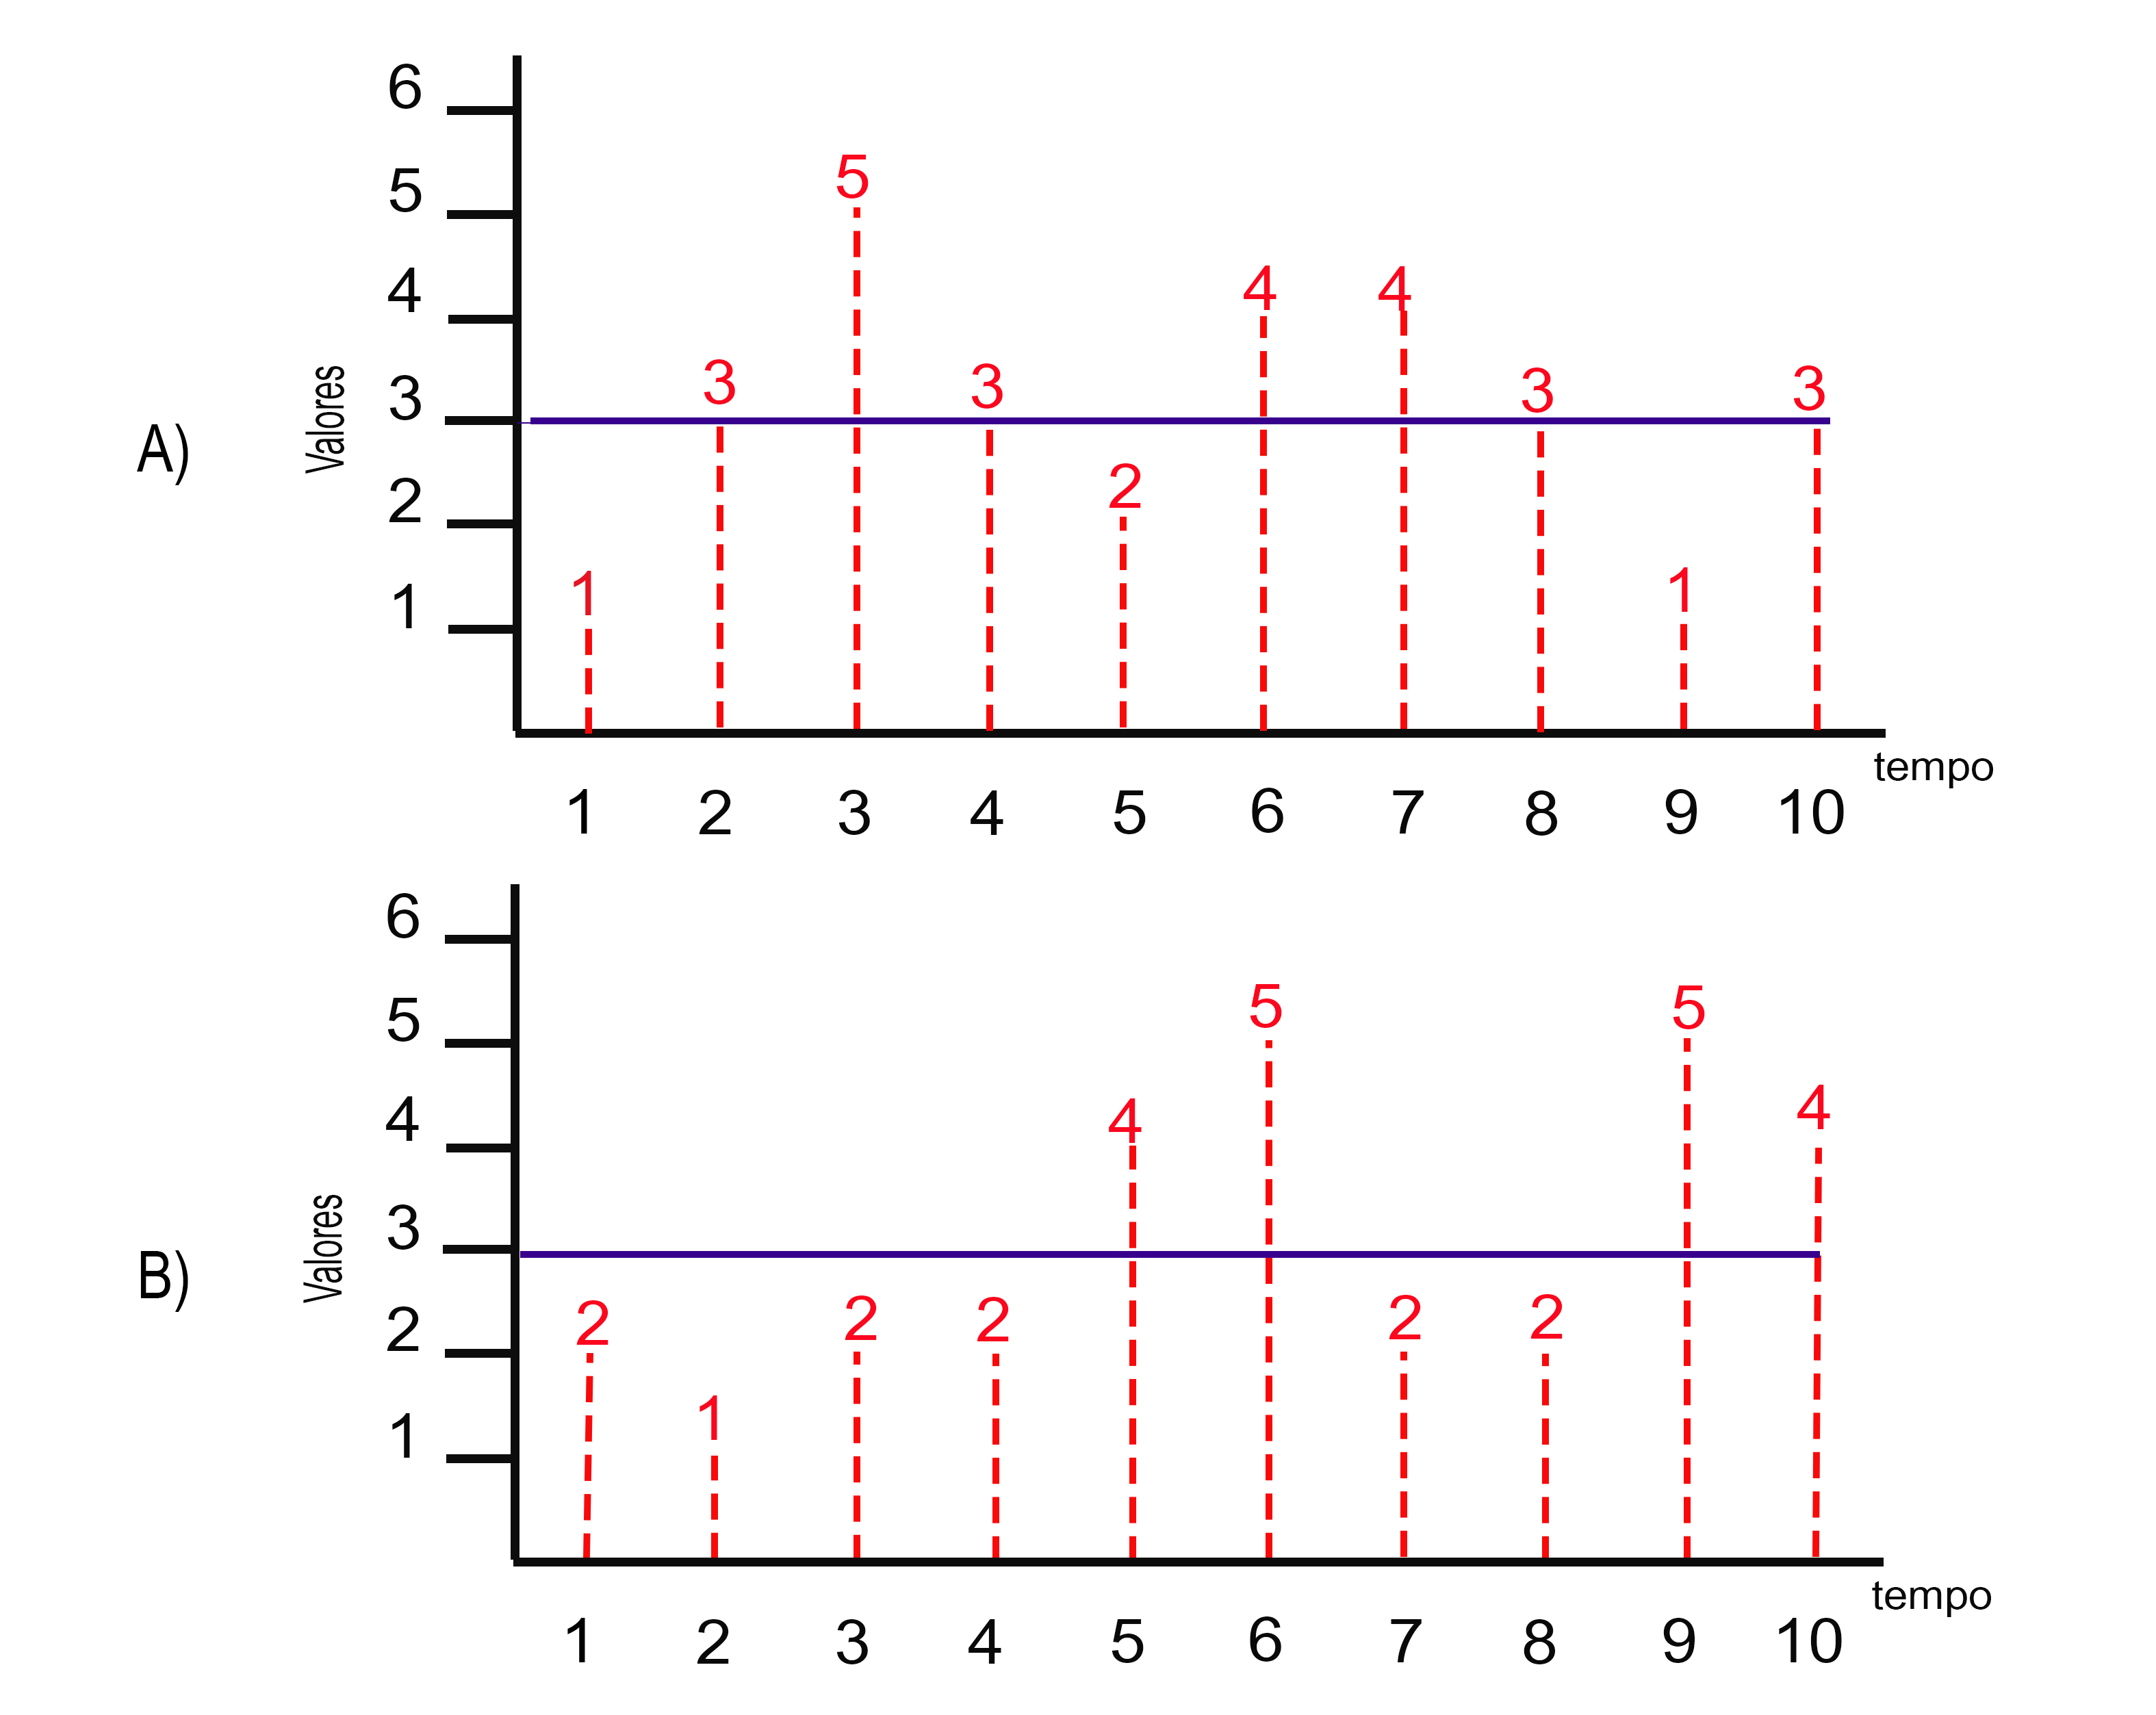
\includegraphics[scale=0.5]{./Capitulo_1/Serie_A.png}	
	\caption{Série de números gerados em A e B. O valor médio destas séries é 2.9.} 
	\label{SerieA}
\end{figure}
\FloatBarrier

Ao observá-los, provavelmente você deve estar imaginando que foram feitos jogando-se dados na mesa. As séries A e B possuem média muito próxima do que seria de um dado de seis lados, e variam de 1 a 6. Na verdade, você está parcialmente certo, eu gerei estes números a partir de dados. A diferença, no entanto, é que a série B foi gerada metade por um dado tetraédrico e metade por um dado cúbico, enquanto os dados da série A foram gerados apenas por um dado cúbico. Os valores médios reais que deveriam ser consideradas para este modelo são os representados na figura \ref{SerieB}. 


\FloatBarrier
\begin{figure}[!htb]
	\centering
	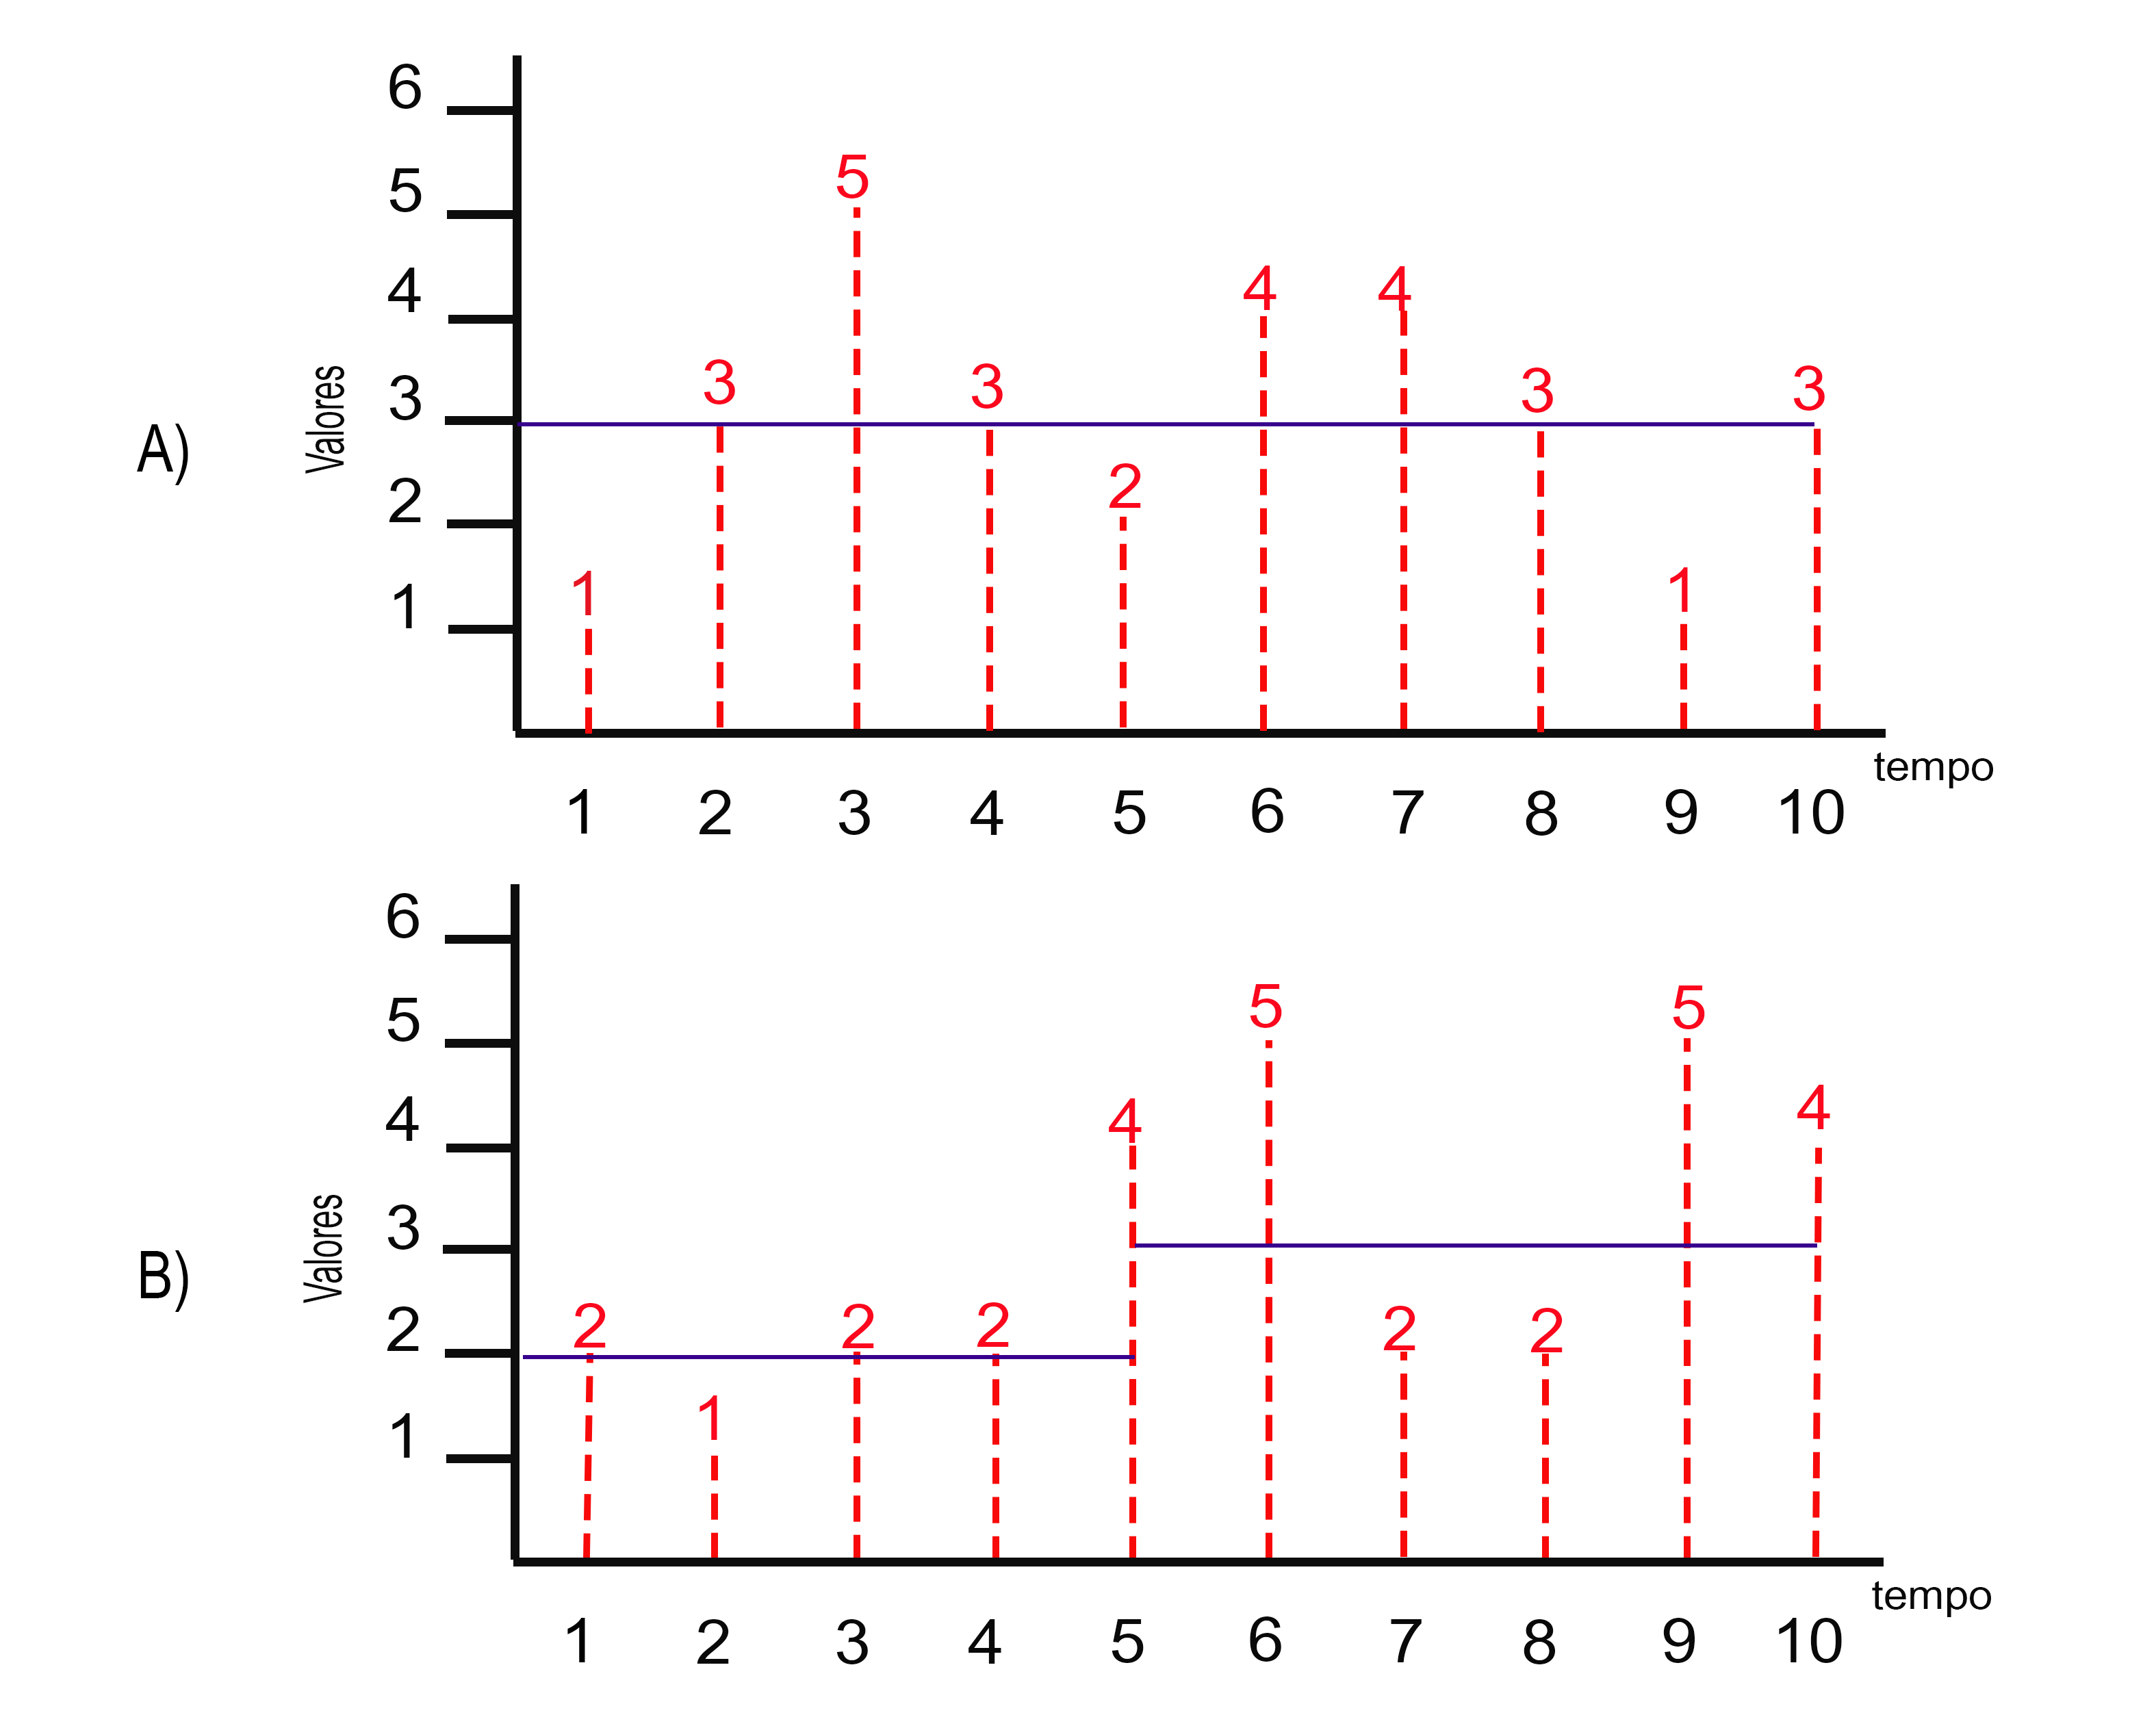
\includegraphics[scale=0.5]{./Capitulo_1/Serie_B.png}	
	\caption{Série de números gerados. Em A) os dados foram gerados a partir de um dado tetraédrico, enquanto em B) foram gerados por um dado cúbico. Apesar dos valores médios globais serem idênticos, as médias locais são diferentes.} 
	\label{SerieB}
\end{figure}
\FloatBarrier

Apesar das médias globais serem exatamente as mesmas, as séries locais possuem distribuições distintas, com média e variância diferentes. Na verdade tanto a série B como série A poderiam ter sido geradas com o mesmo dado de seis lados. A diferença clara, quando consideramos cálculos \textbf{probabilísticos} com cálculos \textbf{estatísticos}, é que a probabilidade requer conhecimento sobre o fenômeno gerador, enquanto a estatística pretende inferir situações a partir das informações dos \textbf{dados}. Na verdade, a única informações que temos a todo momento no depósito mineral são amostras e informações indiretas como geofísica e geoquímica. 

\begin{remark}
	\textit{A decisão de observar uma configuração particular dos dados como estacionário como o resultado de uma função aleatória estacionária está fortemente ligada com a decisão de que estas amostras podem ser unidas juntas. Nenhuma destas decisões pode ser checada quantitativamente, não são certas ou erradas e nenhuma prova das suas validades é possível. No entanto podem ser julgadas como apropriadas ou não.} \citet{isaaks1989applied}
\end{remark}

Apesar de o fenômeno gerador ser completamente distinto para a metade dos dados na série B, não é custoso unir estas diferentes distribuições sobre a mesma hipótese comum. Desta forma, assumir a estacionaridade neste caso é válido, dado que não conhecemos como estas informações foram construídas. 

Em alguns casos, no entanto, não parece ser muito sábio adotar a hipótese de estacionaridade de segunda ordem. Observe a imagem da figura \ref{nonest}. A série é crescente com diferenças de valores iguais a 1 começando de um ${1,2,3,4,5}$. Se você perguntasse para uma criança qual seria o próximo número na sequência ela diria $6$. Se utilizássemos geoestatística para estimar o próximo número considerando a estacionaridade dos valores, o resultado seria $3$.  

\FloatBarrier
\begin{figure}[!htb]
	\centering
	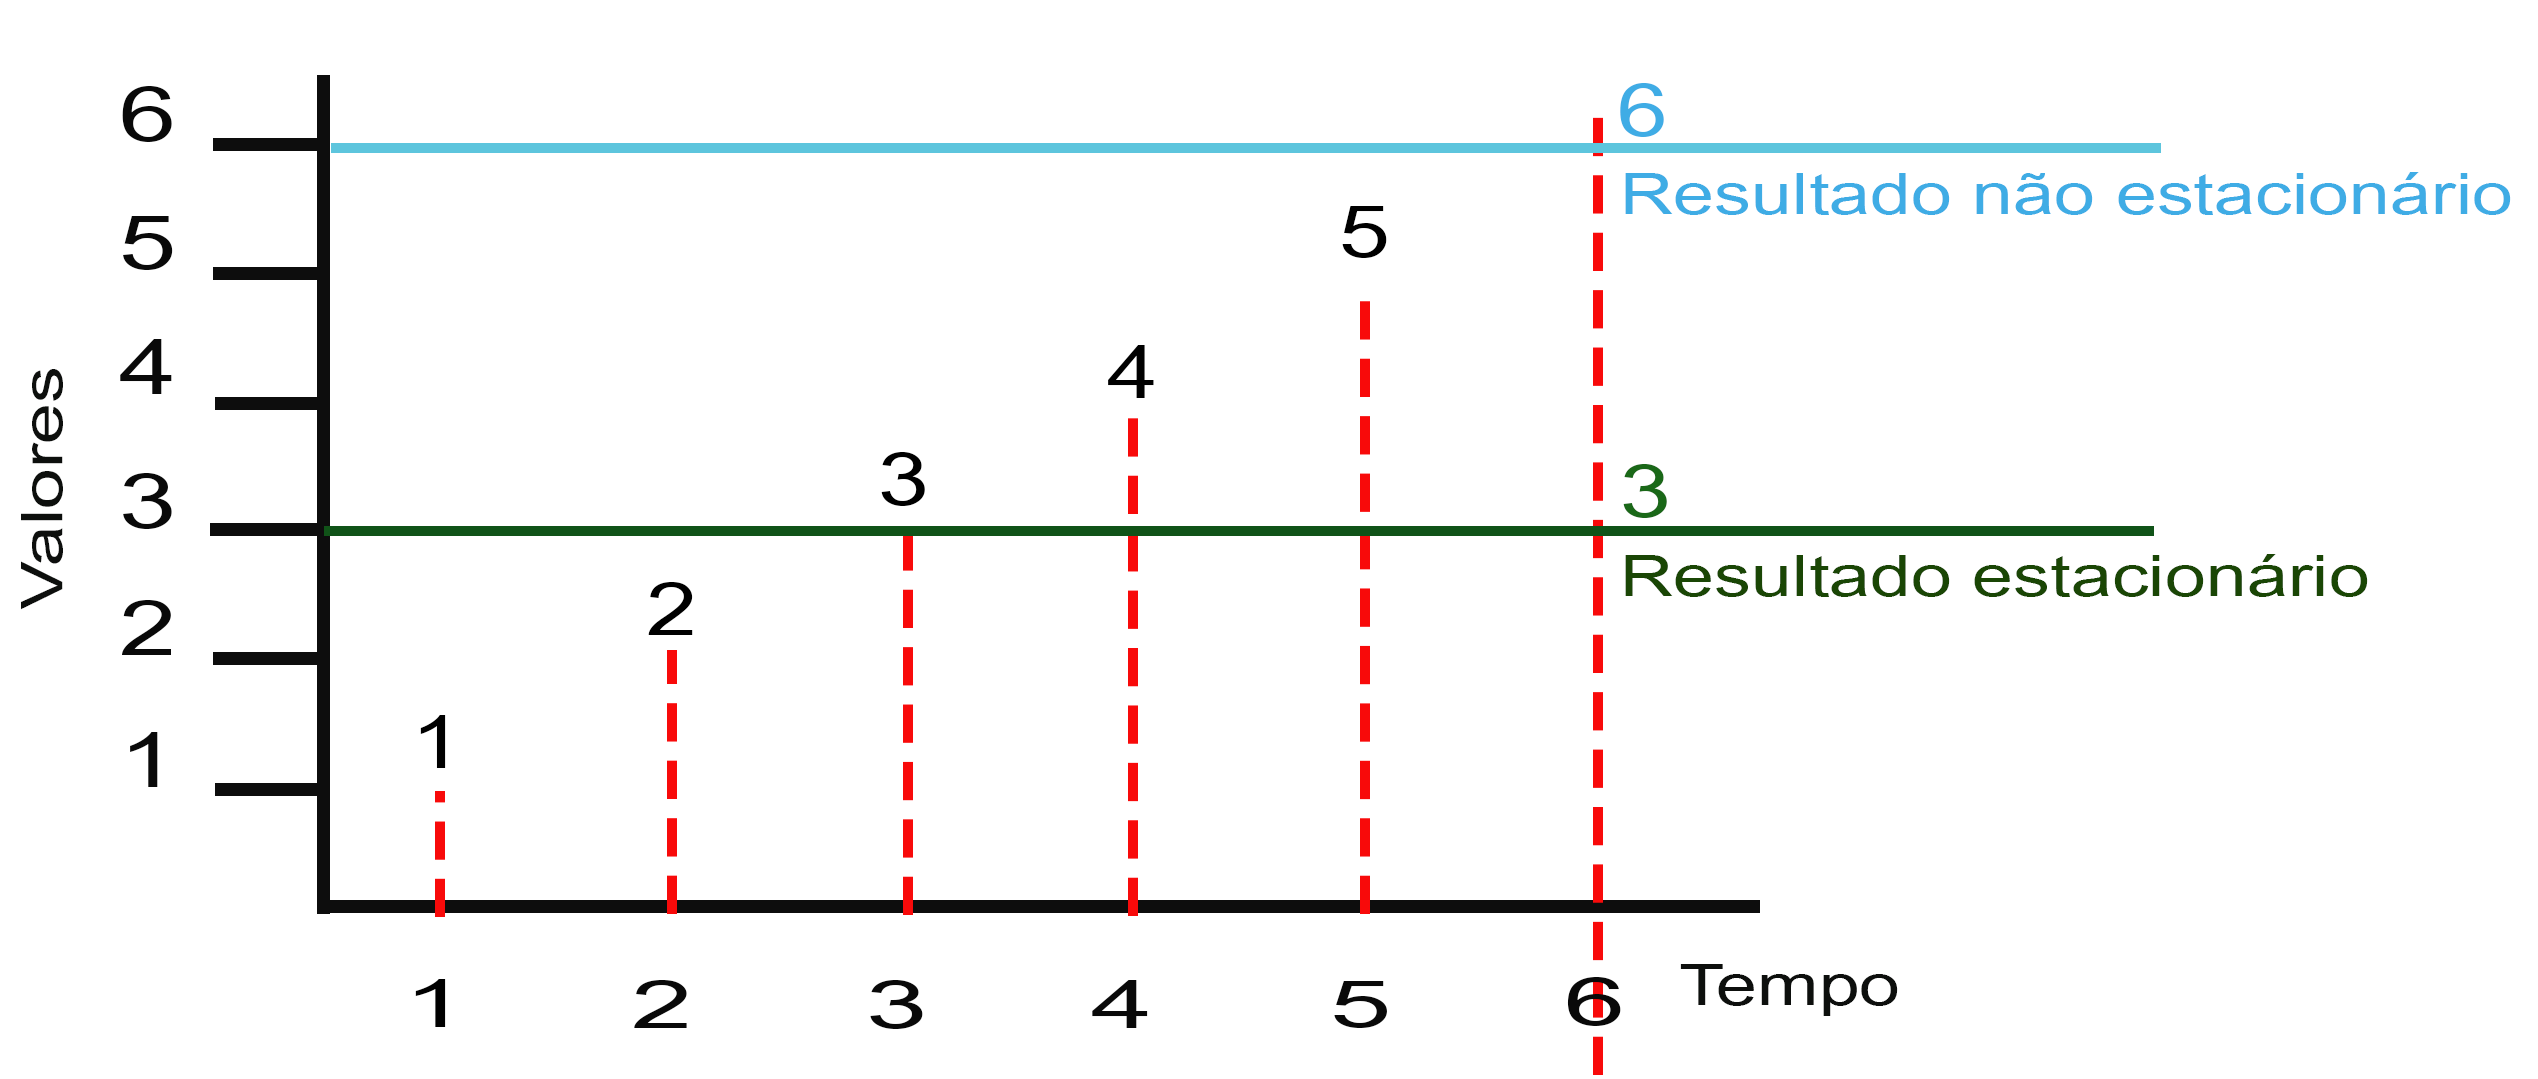
\includegraphics[width=\textwidth]{./Capitulo_1/estacionario.png}	
	\caption{Série crescente de números. O próximo número da sequência a ser estimado considerando um modelo não estacionário seria 7, enquanto para o modelo estacionário seria de apenas 6 } 
	\label{nonest}
\end{figure}
\FloatBarrier

Não parece ser sábio adotar o número 3 neste caso. Se o fenômeno gerador desta série fosse realizado por um dado, seria tão equiprovável encontrarmos o número 3 ou o número 6 na próxima realização. No entanto a informação condicionada pela série parece nos instruir com clareza que existe este padrão a partir da observação indireta dos dados, nós desconhecemos como estes dados foram gerados. Utilizando a geoestatística nos reconhecemos que existe uma \textbf{estruturação} presente nesta sequência, que condicionalmente os dados gerados parecem seguir uma ordem, e que o próximo número gerado tente a apresentar uma variação talvez equivalente como ao dos anteriores, podendo ser 4 ou até mesmo 6.

\begin{remark} 
	\textit{Uma das ideias mais importantes na geoestatística é considerar que a função aleatória gera variáveis aleatórias condicionadas ao longo do espaço. A ideia de continuidade implica que qualquer informação próxima tende a ser mais parecida do que informações muito distantes. Isto é fisicamente plausível, principalmente quando pensamos na geologia. As rochas que estão próximas tendem a possuir propriedades físico-químicas muito mais semelhantes do que quando consideramos uma distância muito grande. Por isso nos é intuitivo considerar o número estimado como 6 e não 3, pois ele representa um comportamento condicionado por medidas sucessivas, logo $Pr\{Z(x_{6}) = 6|z(x_{1}) = 1, z(x_{2}) = 2, z(x_{3}) = 3, z(x_{4}) = 4, z(x_{5}) = 5\} >  Pr\{Z(x_{6}) = 3|z(x_{1}) = 1, z(x_{2}) = 2, z(x_{3}) = 3, z(x_{4}) = 4, z(x_{5}) = 5)\}$ }
	
\end{remark}

Estes casos também são chamados na geoestatística de \textbf{deriva}, ou seja, que existem mudanças graduais na tendência dos dados. Em alguns casos é bastante lógico na mineração considerar a deriva. A topografia, por exemplo, quando analisada em determinadas escalas e situações pode ser continuamente ascendente ou descendente. Neste caso descartar a hipótese de estacionaridade de segunda ordem é sábio. 

\begin{remark}
	\textit{O custo de aceitar o uso de um modelo inapropriado é que as propriedades estatísticas dos valores estimados divergirão de modelos homólogos} \citet{isaaks1989applied}
\end{remark}

\section{Hipótese de estacionaridade} 

Como visto anteriormente podemos realizar hipóteses a respeito da função aleatória, geradora dos fenômenos geoestatísticos. Estas hipóteses são decisões que não podem ser numericamente definidas, mas que em casos convém serem julgadas, para que as estimativas não retornem valores não condizentes com a realidade. A escolha de um tipo de estacionaridade significa que adotamos um critério que considere um conjunto de dados com um comportamento \textbf{homogêneo}. Uma das hipóteses utilizada pela geoestatística mais importantes, e que não constitui critério de escolha, é a chamada de \textbf{hipótese estrita}. Diferentemente da hipótese de estacionaridade de segunda ordem, esta é adotada automaticamente quando se opta por um método geoestatístico e não é passível de decisão. A principal ideia da estacionaridade estrita é que o fenômeno é homogêneo em uma mesma direção no espaço, sendo \textbf{invariante por translação}. 

\begin{remark}
	\textit{A ideia de areia em um jarro é uma boa imagem da estacionaridade de uma função aleatória em três dimensões, pelo menos enquanto a areia estiver bem ordenada (de outra forma se esta jarra vibrar, os grãos finos se depositarão na base, criando não estacionaridade vertical)} \citet{chiles2009geostatistics}
\end{remark}

Uma forma geométrica de pensarmos na hipótese estrita é pelo uso de fractais. Fractais são figuras geométricas autosimilares, em que cada um de seus componentes carregam características da informação como um todo. A figura \ref{fractal} representa um fractal. Estas formas autosimilares são muito comuns na natureza, seja no padrão desenhado por cristais de gelo, pela forma das plantas e principalmente nas rochas. A geologia em pequena escala muitas vezes é uma repetição que se traduz em grande escala. 


\FloatBarrier
\begin{figure}[!htb]
	\centering
	\includegraphics[scale=0.6]{./Capitulo_1/fractal.png}	
	\caption{Fractal gerado a partir da repetição sistemática de estruturas cada vez menores. } 
	\label{fractal}
\end{figure}
\FloatBarrier

\begin{proposition}
	\textit{Todo o conhecimento humano somente advém do entendimento de padrões. As diferentes disciplinas, sejam elas humanas, biológicas ou exatas, apenas diferenciam quanto ao objeto de estudo. Não há diferença nenhuma entre um físico que entende padrões referentes ao movimento de planetas, um linguista que estuda o padrão de idiomas, um historiador que verifica padrões no tempo, ou um matemático que verifica o padrão das formas. A natureza também age desta forma, pois esperamos acordar no dia seguinte com o sol sobre as montanhas. Até mesmo dentro de fenômenos que parecem ser puramente aleatórios, podemos encontrar motivos pelos quais podemos entender padrões. Independente de fenômenos serem estacionários ou não estacionários, a geoestatística procura simplesmente estas formas no espaço, representações que apesar de não serem físicas, são mímicas da natureza da existência destes fenômenos}
\end{proposition}
 
Esta repetição de comportamentos em uma direção leva a seguinte defnição matemática. Um fenômeno dito estacionário estrito significa que $Pr\{Z(x_{1}) < z(x_{1}), Z(x_{2}) < z(x_{2}),..., Z(x_{k}) < z(x_{k})\} = Pr\{Z(x_{1 + h}) < z(x_{1 + h}), Z(x_{2 + h}) < z(x_{2 + h}), ...,Z(x_{k + h}) < z(x_{k  + h})\}$, sendo $h$ um vetor de direção determinada. A hipótese de estacionaridade estrita significa que exite um grau de repetição no comportamento da variável ao longo de uma direção, no entanto, o fenômeno espacial pode apresentar deriva. Outra questão a ser abordada é o fato de que a adoção da estacionaridade é dependente da escala analisada. Um fenômeno considerado não estacionário pode assumir comportamento estacionário local. Obeserva a série de dados representada pela figura \ref{temd}. Quando analisado o comportamento global da função aleatória esta apresenta nitidamente uma tendência nos dados, no entanto, quando considerada uma escala menor do vetor $h$, este mesmo comportamento pode ser tomado como estacionário. Este fenômeno também é chamado de \textbf{quasi estacionário}.


\FloatBarrier
\begin{figure}[!htb]
	\centering
	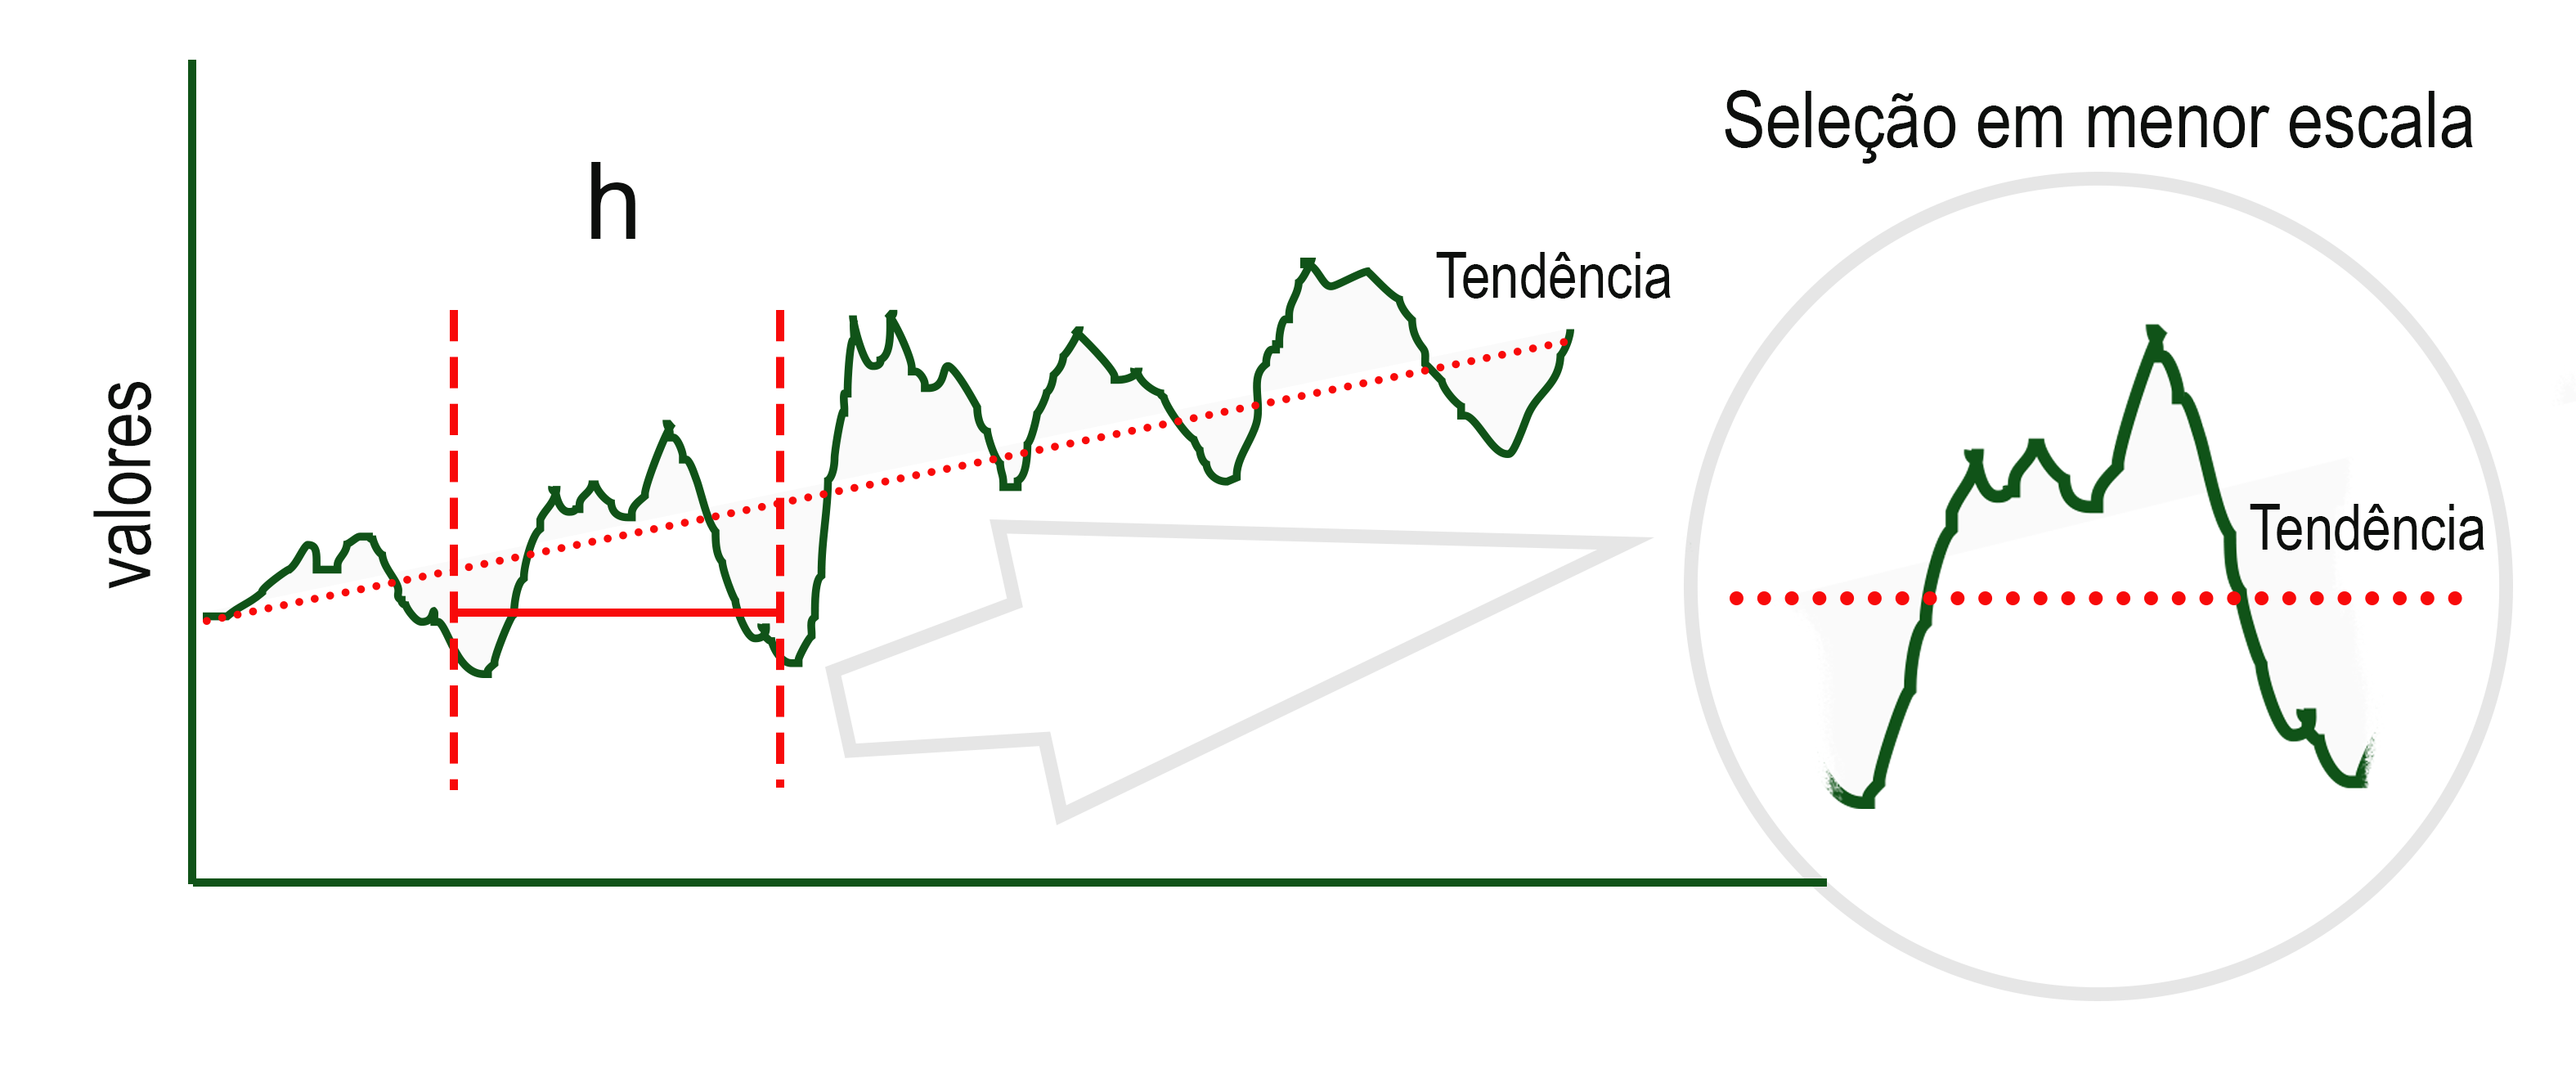
\includegraphics[scale=0.6]{./Capitulo_1/temd.png}	
	\caption{Comportamento analisado de uma série não estacionária quando analisada em um domínio global, e estacionária quando analisada em um domínio menor de comprimento $h$. } 
	\label{temd}
\end{figure}
\FloatBarrier

\begin{proposition}
	\textit{Uma das maiores contribuições da geoestatística para a ciência talvez tenha sido a concepção de que os fenômenos podem ser dependentes da escala analisada. Dependendo da observação nossas hipóteses a respeito do fenômeno podem mudar. Isto é fisicamente compatível com a ideia da geologia. Analisar um depósito mineral em uma grande extensão de área, com toda a certeza é diferente quando observamos variações de tamanho centimétrico. A própria observação da Terra quando vista do espaço apresenta belos tons azuis e brancos, mas quando aproximamos a escala de uma região do tamanho de um país, notamos como nossa visão é diferente e muito mais variável.} 
\end{proposition}

A hipótese de estacionaridade estrita é uma hipótese realizada sobre a característica do fenômeno, não dos resultados das amostras. A hipótese de estacionaridade de segunda ordem, no entanto, é uma hipótese relacionada com os \textbf{momentos estatísticos} do fenômeno. A principal ideia dos momentos estatísticos é que eles representam de alguma forma o resumo da distância entre os dados, desta forma quando pensamos na estacionaridade intrínseca, ou na estacionaridade de segunda ordem, pensamos na possível homogeneidade da distância entre os dados. 

O conceito de \textbf{estacionaridade intrínseca}, desta forma, apresenta também outra forma de conceber esta homogeneidade, quando estabelecemos que uma variação $Y_{h}(x) = Z(x+h) -Z(x)$ é estacionária de segunda ordem. Em outras palavras dizemos que existe homogeneidade quando consideramos a diferenças entre variáveis aleatórias geradas pela função aleatória. Segundo \citet{chiles2009geostatistics}, se a hipótese de estacionaridade intrínseca pode ser considerada e não ocorre uma tendência, então o valor médio da função aleatória é constante, e o valor esperado de $Y_{h}(x)$ é zero. 

\section{Momentos estatísticos} 

Como dito anteriormente, momentos estatísticos são representações da distância entre dados. As medidas de distância, podem ser por exemplo, medidas da tendência central dos dados ou medidas da dispersão destes dados. A figura \ref{moment} representa os conceitos de \textbf{tendência central}  e de \textbf{dispersão}. 

\FloatBarrier
\begin{figure}[!htb]
	\centering
	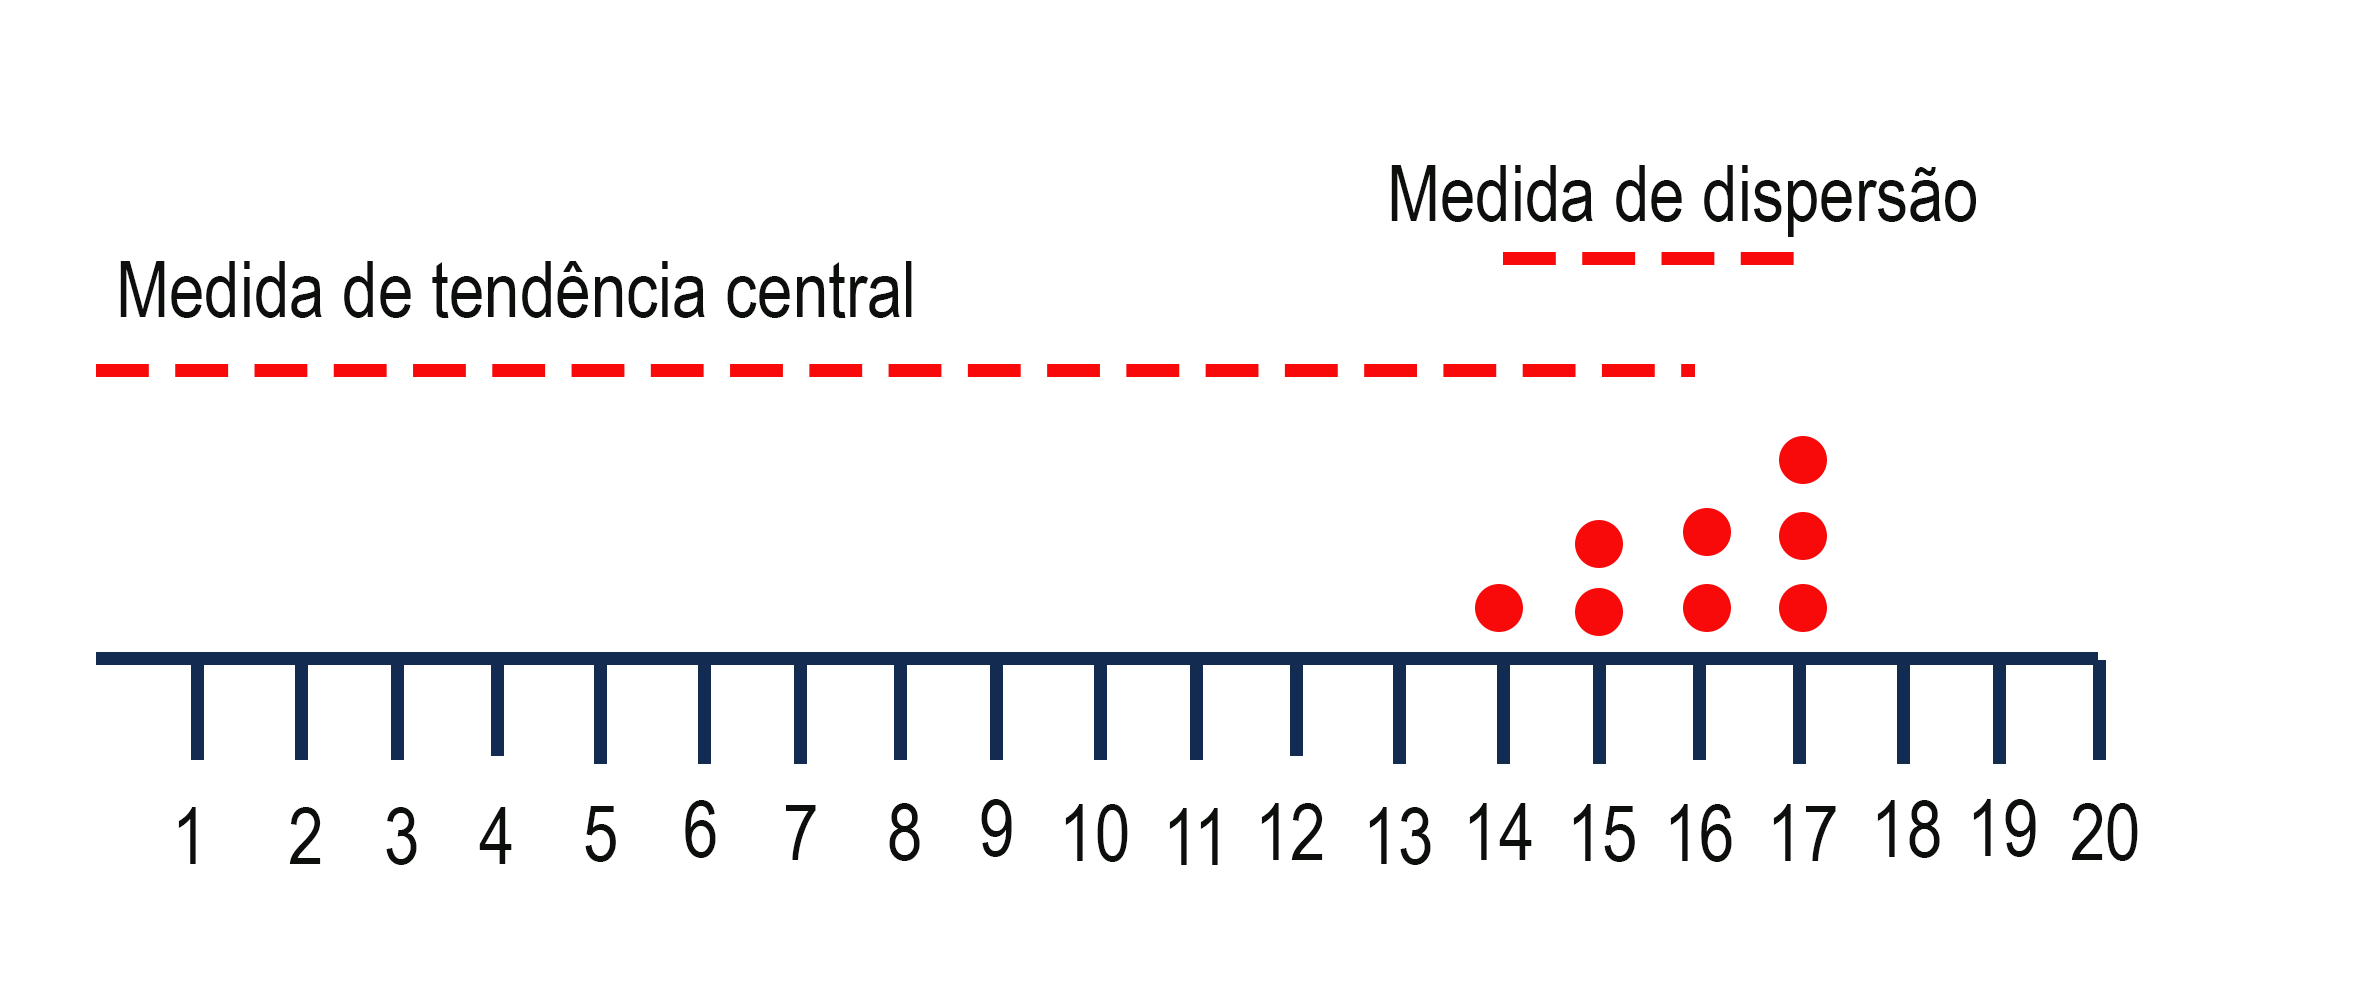
\includegraphics[scale=0.8]{./Capitulo_1/moment.png}	
	\caption{Exemplos de momentos estatísticos para um conjunto de dados. O valor médio representa o quão distante está o centro dos dados, enquanto a dispersão apresenta quão agregados estão estes dados. } 
	\label{moment}
\end{figure}
\FloatBarrier

A principal medida da distância do centro dos dados é chamada de \textbf{esperança matemática}, e pode ser representada para variáveis contínuas como. 

\begin{equation}\label{eq1:Valor_esperado}
E\left(Z\right)= \int_{z = -\infty}^{z =+\infty} z f\left(z\right)dz
\end{equation}

No caso de variáveis discretas, podemos determinar a esperança matemática como 

\begin{equation}\label{eq2:Valor_esperado_discreto}
E\left(Z\right)= \sum_{i=-\infty}^{+\infty}Pr\left(z_i\right)z_i
\end{equation}

Muitas vezes há confusões ao se dizer que a esperança matemática representa o valor mais provável que determinada variável pode possuir. No entanto, a esperança matemática é simplesmente uma medida da distância do centro dos dados, sendo que este centro pode ser pouco provável ou nem mesmo existir. Observe a figura \ref{moment2}. A esperança matemática neste caso representa o centro de uma distribuição com probabilidade muito baixa de ocorrência.

\FloatBarrier
\begin{figure}[!htb]
	\centering
	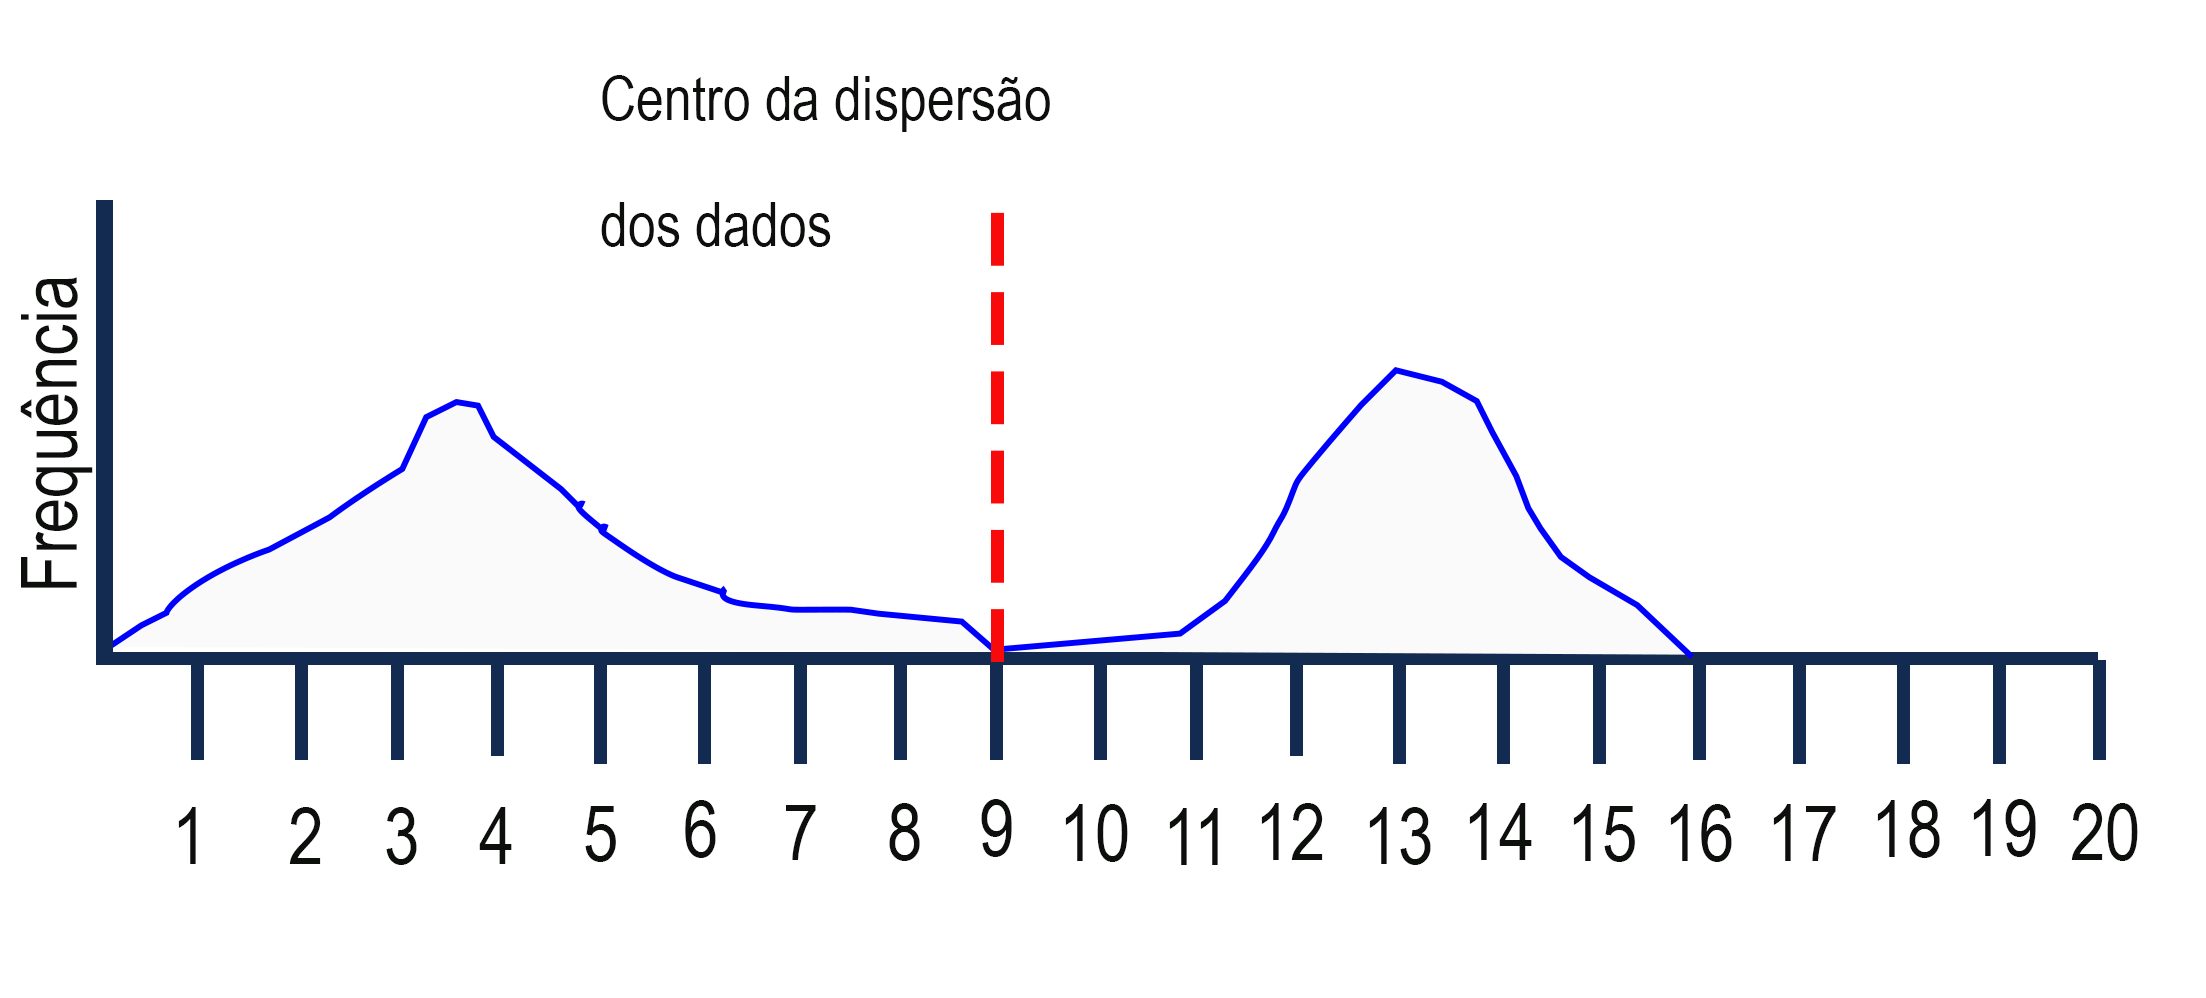
\includegraphics[scale=0.6]{./Capitulo_1/moment2.png}	
	\caption{Exemplo da esperança matemática de uma distribuição multimodal. O valor da probabilidade para este centro de dispersão é praticamente nulo. } 
	\label{moment2}
\end{figure}
\FloatBarrier

O que de fato ocorre é que os centros de dispersão dos dados da maioria dos problemas de engenharia não são multimodais, ou seja, apresentam vários picos nas distribuições de densidade de probabilidade com na figura. Neste caso a esperança matemática pode representar os valores mais prováveis de ocorrência da dispersão dos dados.

Pela definição da esperança matemática, algumas propriedades podem ser diretamente derivadas. A multiplicação da variável aleatória $Z$ por um valor constante $c$, implica na seguinte condição. 

\begin{equation}\label{eq3:Propesperancamatematica}
E\left(cZ\right)= cE\left(Z\right)
\end{equation}

O valor esperado de uma variável aleatória constante pode ser relacionada pela seguinte propriedade

\begin{equation}\label{eq4:Propesperancamatematica2}
 E(c) = c
\end{equation}

A demonstração, na verdade é muito simples, já que advém da própria definição de esperança mamtemática


\begin{proof} 
	Valor esperado de uma constante é igual a ela mesma
	\begin{align*}
	&E\left(c\right)= \sum_{i=-\infty}^{+\infty}Pr\left(c\right)c \\
	& E\left(c\right)= c\sum_{i=-\infty}^{+\infty}Pr\left(c\right) \\
	& Como: \sum_{i=-\infty}^{+\infty}Pr\left(c\right) = 1 \\
	& E\left(c\right)= c
	\end{align*}
\end{proof}

A partir da definição da esperança matemática como uma medida de centralidade da distribuição dos dados, podemos derivar outros momentos representando diferentes distâncias desta distribuição. Os diferentes momentos matemáticos podem caracterizar diferentes distâncias relativas à \textbf{centralidade} , \textbf{dispersão} , \textbf{assimetria} , \textbf{forma}. A geoestatística, na verdade, foca sua análise principalmente nos momentos de primeira e segunda ordem.

\begin{remark}
	\textit{Em aplicações da mineração, a lei de probabilidades espacial nunca é requerida, principalmente porque os dois primeiros momentos da função são suficientes para providenciar uma solução aproximada para muitos problemas encontrados} \citet{journel1978mining}
\end{remark}

Outro momento estatístico importante é a variância, definida como o momento de segunda ordem centrado. A variância pode ser considerada como uma medida de dispersão, demonstrada por

\begin{equation}\label{eq4:CapVariancia1}
Var\left(Z\right)= E\left( Z - E\left( Z\right) \right)^2
\end{equation} 

Esta forma tradicional da variância pode ser substituída por outra representação a partir de 

\begin{equation}\label{eq4:CapVariancia2}
Var\left(Z \right)= E(Z^2) - E(Z)^2
\end{equation} 

fA prova desta relação também é facilmente demonstrada a partir das propriedades da esperança matemática e pela definição da variância.

\begin{proof} 
	Relação entre as equações \ref{eq4:CapVariancia1} e \ref{eq4:CapVariancia2}
	\begin{align*} 
	&Var\left( Z \right)= E\left( Z -E(Z) \right)^2  \\
	&Var\left(Z \right)= E\left( Z^2 -2ZE\left( Z\right)+ E(Z)^2 \right) \\
	&Var\left(Z \right)= E(Z^2) -E(2ZE(Z)) +E(Z)^2  \\
	&Var\left(Z \right)= E(Z^2) -2E(Z)E(Z) +E(Z)^2  \\
	&Var\left(Z \right)= E(Z^2) -2E(Z)^2 +E(Z)^2 \\
	&Var\left(Z \right)= E(Z^2) - E(Z)^2
	\end{align*}
\end{proof}

 Os momentos estatísticos de primeira e segunda ordem, representados pela esperança matemática e pela variância representam medidas tomadas de uma única variável aleatória. Para relacionar diferentes variáveis aleatórias utilizamos comumente a \textbf{covariância}, esta representada pela similaridade entre duas variáveis aleatórias. Considere as variáveis aleatórias Z e Y. Podemos representar a covariância pela seguinte relação
 
 \begin{equation}\label{eq6:CapCorrelacao}
 Cov\left(Z,Y\right)= E\left( (Z-E(Z)) (Y-E(Y)) \right)
 \end{equation}
 
 Se as variáveis $Z$ e $Y$ apresentam médias idênticas iguais a $m$, então a covariância pode ser representada por 
 
  \begin{equation}\label{eq6:CapCorrelacao}
 Cov\left(Z,Y\right)= E\left( ZY \right) - m^{2}
 \end{equation}
 
 A prova desta relação pode ser facilmente obtida 
 
 \begin{proof}
 	Relação da Covariância considerando médias idênticas iguais a m
 	\begin{align*}
 	&Como:  E(Z) = E(Y) = m  \\
 	&Cov\left(Z,Y\right)= E\left( (Z-m) (Y-m) \right)\\
 	&Cov\left(Z,Y\right)= E\left( ZY - Zm - Ym +m^2 \right)\\
 	&Cov\left(Z,Y\right)= E(ZY) - E(Zm) - E(Ym) +E(m^2)\\
 	&Cov\left(Z,Y\right)= E(ZY) - mE(Z) - mE(Y) +E(m^2)\\
 	&Cov\left(Z,Y\right)= E(ZY) - m^2 - m^2 +m^2\\
 	&Cov\left(Z,Y\right)= E(ZY) - m^2
 	\end{align*}
 \end{proof}

Se as variáveis Y e Z forem idênticas, a covariância entre as duas variáveis aleatórias é equivalente a variância. A prova pode ser demonstrada por

\begin{proof}
	Prova de que a covariância é idêntica a variância para Z=Y
	\begin{align*}
	&Como: Y=Z \rightarrow Cov(Z,Y) = Cov(Z,Z)  \\
	&C\left(Z,Z\right) = E\left( (Z-E(Z))(Z-E(Z)) \right) \\
	&C\left(Z,Z\right) = E\left( Z-E(Z) \right)^2 \\
	&C\left(Z,Z\right) = Var(Z) \vee   Var(Y) \\
	\end{align*}
\end{proof}

\section{Ergocidade} 

A ergocidade é uma das propriedades mais importantes da funcão aleatória. A ideia é de que cada vez ao qual analisamos um volume maior no espaço, a tendência é que o valor médio deste volume se aproxime cada vez mais do valor médio do fenômeno. Matematicamente podemos definir a propriedade da ergocidade como 

\begin{equation}
\lim_{V\rightarrow \infty}\frac{1}{|V|}\int_{x \in V}Z(x)dx = m 
\end{equation}

Em que $|V|$ é o volume considerado e $m$ o valor da média do fenômeno. 
\begin{definition}[Ergocidade]
	\textit{A Ergocidade pode ser caracterizada como a propriedade da função aleatória de convergência dos valores médios se aproxime a um valor constante $m$, de acordo com um domínio $V$ considerado.}
\end{definition}

Alguns fenômenos tendem a apresentar dispersões infinitas, crescentes de acordo com o desenvolvimento da função aleatória. Estes fenômenos podem apresentar dispersão infinita, tal como o fenômeno de movimento browninano. 

\section{Homocedasticidade e heterocedasticidade}

Além do comportamento da estacionaridade dos valores médios da função aleatória, também é importante qualificar os fenômenos geoestatísticos a partir do comportamento da variância. A figura \ref{etero}, por exemplo, demonstra um comportamento crescente da variância de acordo com o desenvolvimento da série.

\FloatBarrier
\begin{figure}[!htb]
	\centering
	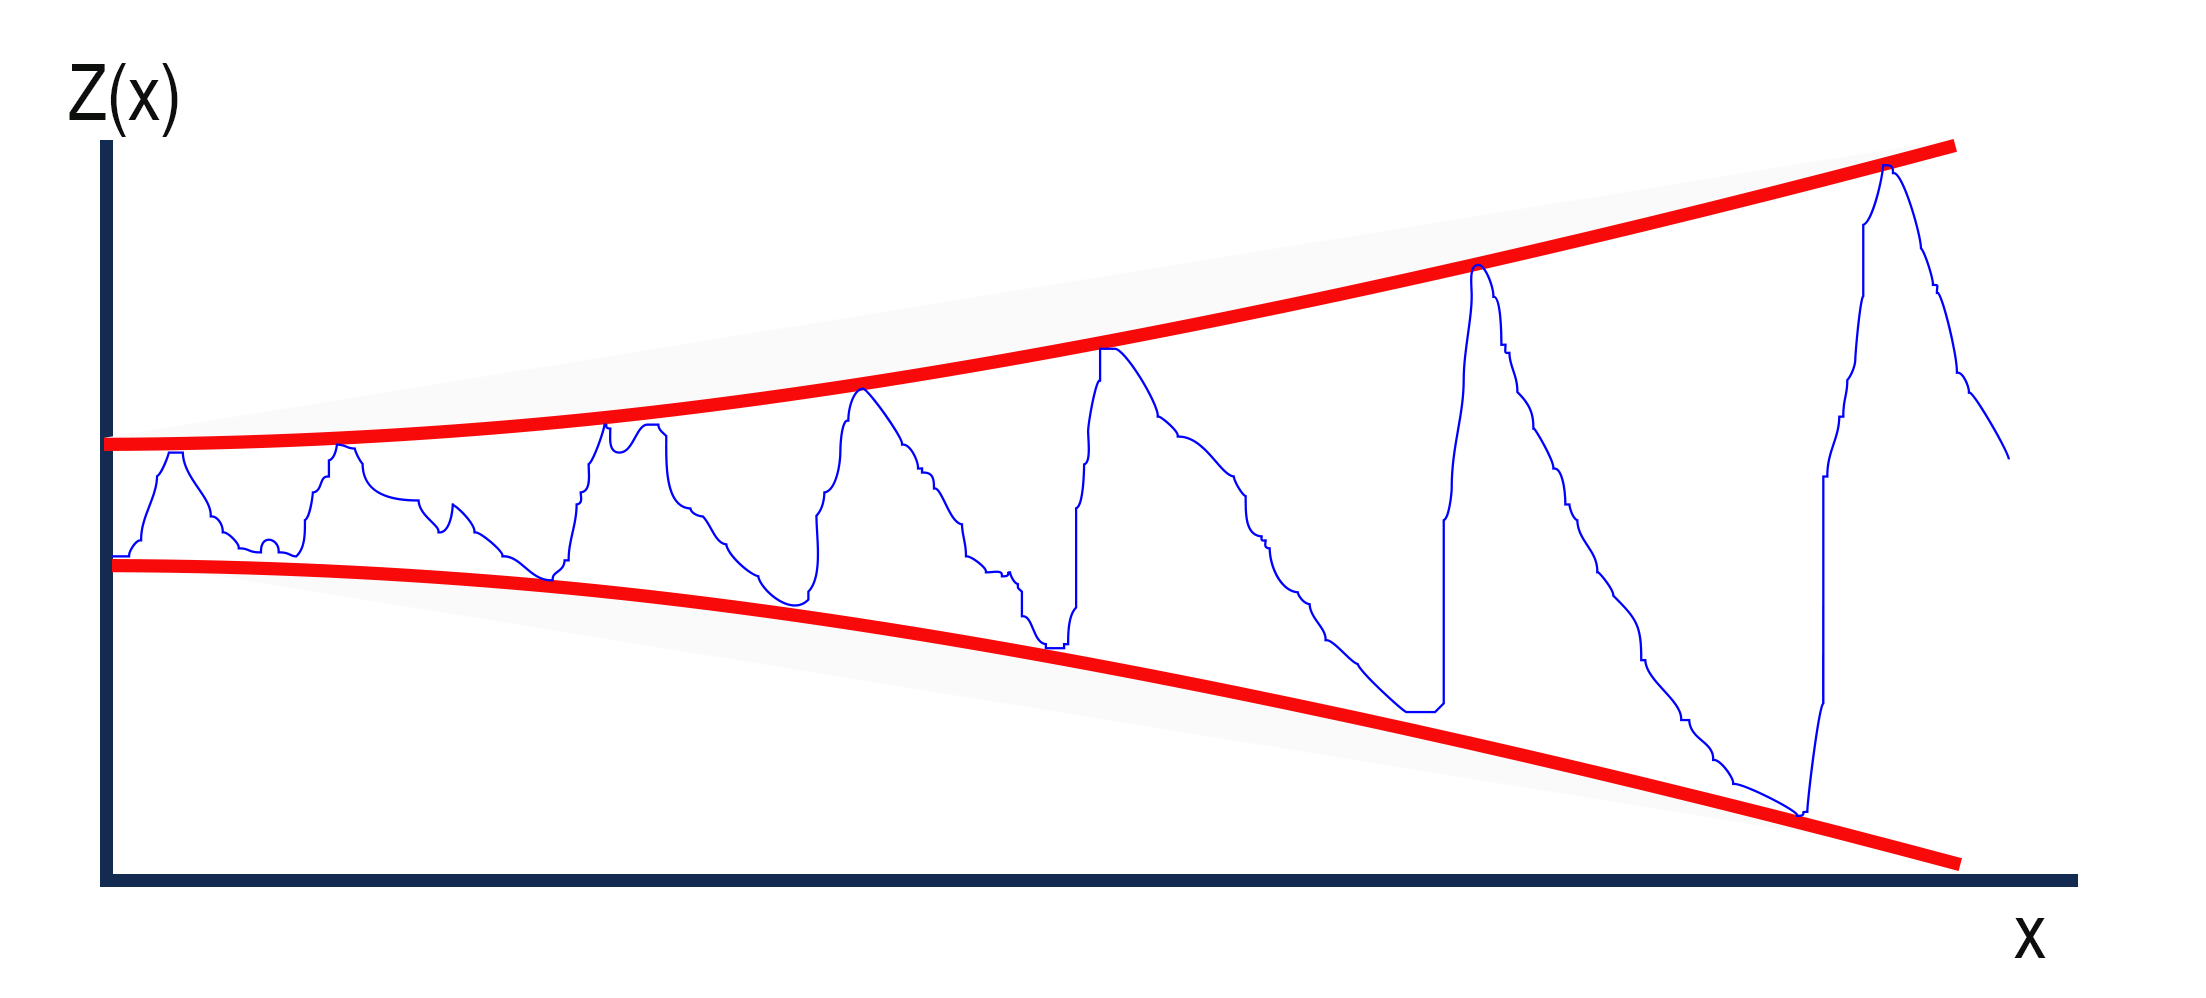
\includegraphics[width=\textwidth, height=4cm]{./Capitulo_1/heterocedasticidade.png}	
	\caption{Fenômeno de heterocedasticidade representando variabilidade infinita da função aleatória } 
	\label{etero}
\end{figure}
\FloatBarrier

 Estes fenômenos são chamados de \textbf{heterocedásticos}, e aumentam a variabilidade de acordo com o incremento da direção. Fenômenos constantes quanto a dispersão local são chamados de \textbf{homocedásticos}

\begin{definition}[homocedasticidade]
	A hipótese de homocedasticidade,  igual \textit{(homo)} dispersão \textit{(scedasticidade)}, implica que a variância da função aleatória é constante para todo e qualquer ponto $x$ representado no domínio $D$. A heterocedasticidade, no entanto, implica que a variância aumenta ao longo da função aleatória.
\end{definition}

\section{Relação Volume Variância}

Na geoestatística, a variável aleatória se manifesta em todos os pontos no espaço. No entanto, nem sempre é possível reconhecer a variável em um suporte pontual, e para fins de engenharia precisamos entender a variável aleatória dentro de domínios específicos, sejam eles os domínios da amostra, na unidade seletiva de lavra, ou dentro de um domínio de estimativa. Na geoestatística clássica, apenas se determina os \textbf{valores esperados} destas variáveis dentro de um domínio, principalmente os de primeira e segunda ordem, não se importando com o reconhecimento das distribuições locais. 

O processo de se determinar volumes esperados dentro de um domínio é chamado na geoestatística de \textbf{regularização}. 

\begin{remark}
	\textit{Muito raramente, em prática, o valor dos dados pontuais $z(x)$ estão disponíveis. Mais comumente o valor dos dados $z_{v}(x)$ em um certo suporte $v(x)$ estão disponíveis, como por exemplo uma amostra de testemunho, ou mais genericamente o volume de uma amostra. O valor médio $z_{v}(x)$ é chamado de regularização das variáveis pontuais $z(y)$ dentro do domínio $v(x)$ } \citet{journel1978mining}
\end{remark}

A regularização permite com que medidas realizadas dentro de um domínio estipulado possuam mesmo volume, permitindo com que suas propriedades sejam compatíveis para fins de estimativa na geoestatística. 

Assumindo que a função aletória é contínua, e que uma combinação linear de variáveis aleatórias pode ser expressa, podemos definir um valor regularizado em um espaço amostral, definido pelo seu suporte. Considere $v$ como o suporte amostral, logo o seu valor regularizado pode ser descrito como

\begin{equation}
Z_{v} = \frac{1}{|v|}\int_{x\in v} Z(x)dx
\end{equation}

Da mesma forma o valor regularizado dentro da unidade seletiva de lavra pode ser definido por 

\begin{equation}
Z_{V} = \frac{1}{|V|}\int_{x\in V} Z(x)dx
\end{equation}

Em último caso podemos definir o valor médio dentro do domínio de estimativa

\begin{equation}
Z_{D} = \frac{1}{|D|}\int_{x\in D} Z(x)dx = m
\end{equation}

Em que $m$ é o valor esperado do fenômeno considerado, e constante, se considerada a propriedade da ergocidade. Considerando os diferentes domínios $v$, $V$, e $D$, podemos determinar três diferentes relações $(v|V)$, $(v|D)$ ou $(V|D)$, representadas pelas relações entre amostras e unidade seletiva de lavra, amostras e domínio de estimativa e unidades seletivas de lavra e domínio de estimativa.   


Para indicarmos a variabilidade ao qual os valores amostras em um domínio estão dispersos quanto um valor de referência estimado, utilizamos uma estatística chamada de \textbf{variância de dispersão}, denotada pela letra $D^{2}$. A ideia da variância está diretamente associada ao conceito de \textbf{entropia}, ou grau de desorganização. 

\begin{proposition}
	\textit{A variância de dispersão é uma das medidas mais importantes na geoestatística e está associada ao conceito de entropia, ou de desorganização dos dados. Quando você considera, por exemplo, a variabilidade de um pixel de uma foto em relação ao seu valor médio, com toda a certeza este será mais disperso que valores médios de partes do corpo na foto, como rostos e mãos, em relação a este valor central. A ideia de que nosso conhecimento sobre um fenômeno pode ser afetado pela dispersão da informação é essencial, principalmente nas técnicas de mudança de suporte que serão vistas futuramente.}
\end{proposition}

A \textbf{variância de dispersão} é portanto uma medida da variabilidade entre estes domínios, considerando os valores regularizados. A variância de dispersão amostra e domínio de estimativa pode ser definida por


\begin{equation}
D^{2}(v|V) = \frac{1}{N}\sum_{i \in V}[Z_{v_{i}} - Z_{V}]^{2}
\end{equation}

Sendo N o número de pontos amostrais regularizados de suporte $v$ dentro do domínio estimado $V$. Se considerarmos o suporte $(.)$ como o suporte pontual, podemos definir a variância de dispersão ponto amostra por 

\begin{equation}
D^{2}(.|v) = \frac{1}{|v|}\sum_{x \in v}[Z(x) - Z_{v}]^{2}
\end{equation}

Em que $|v|$ é o volume constituído pelo suporte amostral $v$ e todos os seus pontos internos. E a variância de dispersão ponto e domínio estimado por 

\begin{equation}
D^{2}(.|V) = \frac{1}{|V|}\sum_{x \in V}[Z(x) - Z_{V}]^{2}
\end{equation}

Em que $|V|$ é o volume constituído pelo suporte amostral $V$ e todos os seus pontos internos. Uma das relações importantes da variância de dispersão pode ser determinada pela diferença entre variâncias de dois suportes, tal como
\begin{proof}
	Prova da relação da variância de dispersão entre ponto e bloco estimado como a diferença entre a variância do fenômeno e da variância do bloco estimado.
	\begin{align*}
	&D^{2}(.|V) = \frac{1}{|V|}\sum_{x \in V}[Z(x) - Z_{V}]^{2}  \\
	&D^{2}(.|V) = \frac{1}{|V|}\sum_{x \in V}[Z(x)^{2} - 2 Z(x)Z_{V} + Z_{V}^2] \\
	&como \sum_{x \in V} Z(x)Z_{V} = Z_{V}^2, \text{tal que } Z_{V} = constante\\
	&D^{2}(.|V) = \frac{1}{|V|}\sum_{x \in V}[Z(x)^{2} - Z_{V}^2]  \\
	&D^{2}(.|V) = \frac{1}{|V|}\sum_{x \in V}([Z(x)^{2} - m^{2} - (Z_{V}^2 - m^{2})] \\
	&\text{Pela hipótese de estacionaridade de segunda ordem:}  \\
	&\frac{1}{|V|}\sum_{x \in V}[Z(x)^{2} - m^{2}] = Var(Z(x)) = s^{2}(.|.)\text{ , e}\\
	&[Z_{V}^2 - m^{2}] = Var(Z(V)) = s^{2}(V|V)\text{ , logo}\\
	&D^{2}(.|V) = D^{2}(.|.) - D^{2}(V|V)  \\
	\end{align*}
\end{proof}

Analogamente as relações $s^{2}(.|v) = s^{2}(.|.) - s^{2}(v|v)$ e $s^{2}(v|V) = s^{2}(V|V) - s^{2}(v|v)$ podem ser derivadas. Podemos encontrar então a seguinte identidade 

\begin{equation}
s^{2}(.|V) = s^{2}(.|v) + s^{2}(v|V)
\end{equation}

Esta também é chamada de \textbf{relação de krige} ou relação da aditividade de variâncias de krige. Quando consideramos a dispersão de valores de uma variável em domínios maiores como $V$, esta tende a ser maior que consideramos no suporte amostral $v$. Este princípio também é chamado de \textbf{volume e variância}, ou seja, quanto maior for a diferença entre os suportes amostrais e o domínio de estimativa, menor será nossa acurácia nestas predições. A ideia da variabilidade de acordo com a mudança do volume estimado ou do suporte amostral está diretamente associada à definição de uma imagem, no conceito da geoestatística.  Observe a figura \ref{volume_var}. Em A) possuímos os valores exaustivos do fenômeno estudado. Podemos notar que os resultados são uma representação fiel de uma representação física, podem ser realmente consideradas um "mapa" dos valores distribuídos no espaço. Em B) verificamos os valores estimados, que se apresentam de forma pixelada e não apresentam uma definição adequada do problema. No entanto, cada bloco estimado no mapa B) guarda uma correlação alta com os valores médios tomados da região no mapa A). Dizemos que as estimativas geoestatísticas não são uma ferramenta boa para produzir "mapas", já que estes são reproduções fidedignas dos fenômenos espaciais, mas o valor esperado dentro de um bloco em B) tende a ser cada vez mais próximo do valor médio real na região quanto menor for a definição e maior o tamanho do bloco. 

\FloatBarrier
\begin{figure}[!htb]
	\centering
	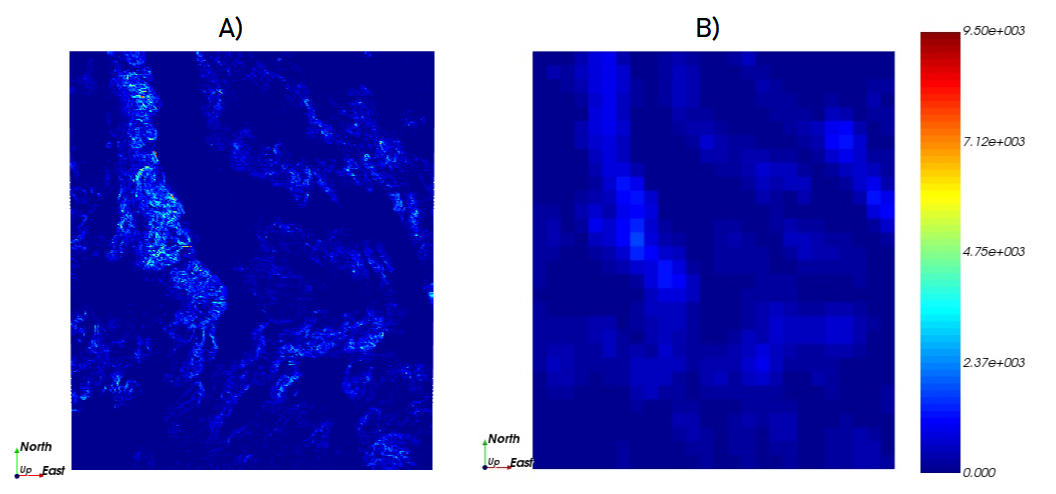
\includegraphics[width=\textwidth]{./Capitulo_1/kriged.png}	
	\caption{Relação do conceito de volume e variância apresentado em imagens. Em A) possuimos o valor exaustivo de um banco de dados, enquanto em B) apresentamos os valores krigados. É possível notar que as estimativas não reproduzem as feições naturais do fenômeno, no entanto, cada bloco estimado é  } 
	\label{volume_var}
\end{figure}
\FloatBarrier



\section{Conclusões} 

Neste capítulo aprendemos um pouco sobre a teoria das variáveis regionalizadas, um conceito determinado na década de 70 pelo professor George Matheron, e que evoluiu ao longo do tempo, facilitando o estudo de variáveis georeferenciadas. Estes conceitos iniciais são abstratos, porém poderosos, pois permitem constituir as bases de hipóteses utilizadas nos modelos geoestatísticos. 


\section{Exercícios}

\begin{exercise}
	Enumere em uma lista todas as variáveis aleatórias regionalizadas que você possui em seu objeto de estudo. Indique ao lado se elas são somáticas ou não. Ex.: Teor-> somático, Condutibilidade hidráulica -> não somático.
\end{exercise}

\begin{exercise}	
 Cinco ações de uma mineradora possuem rentabilidade de 5, 10,20,4 e 5 Unidades monetárias. Se a probabilidade de renda destas ações forem iguais a 40\%, 35\%, 10\%, 10\% e 5\% qual é o valor esperado para a renda de todas as ações. Resp.:8.15 UM
\end{exercise}

\begin{exercise}
	Cinco amostras possuem valor de teor iguais a 2\%, 2.5\%,2.3\%,2.1\% e 2.7\%. Se o volume das amostras é de 5,4,3,5 e 7 $cm^3$ qual é o teor médio das amostras. Resp.: 2,34\%
\end{exercise}
\begin{exercise}	
	\item Prove que o valor do resíduo da função aleatória é ortogonal à sua tendência, ou seja $Cov(R,m) = 0 \forall x \in D$ sendo D o domínio do depósito.
\end{exercise}
\begin{exercise}
	\item Prove que a covariância de duas variáveis aleatórias independentes seja igual a zero. Dica.: Tome o valor de $E(XY) = E(X)E(Y)$
	
\end{exercise}

 